% Báo cáo K03 theo bố cục mẫu "Xử lý tiếng vang trong tín hiệu âm thanh".
% Biên dịch: tectonic bao_cao_k03.tex --outdir .
% Các mục \CanBoSung là thông tin chưa có chứng cứ trong repository; không thay
% bằng kết quả dự đoán. Hình được tạo bởi make_figures.py từ CSV gốc.
\documentclass[14pt,a4paper,oneside]{extreport}
\usepackage[left=30mm,right=20mm,top=20mm,bottom=20mm]{geometry}
\usepackage{fontspec}
\IfFontExistsTF{Times New Roman}{\setmainfont{Times New Roman}}{\setmainfont{Liberation Serif}}
\setsansfont{DejaVu Sans}
\setmonofont{DejaVu Sans Mono}[Scale=0.84]
\usepackage{polyglossia}
\setdefaultlanguage{vietnamese}
\usepackage{amsmath,amssymb,booktabs,longtable,array,multirow}
\usepackage{graphicx,float,caption,subcaption}
\usepackage{setspace}
\usepackage{titlesec,tocloft,needspace}
\usepackage{tikz}
\usetikzlibrary{arrows.meta,positioning,shapes.geometric,calc}
\usepackage{indentfirst}
\usepackage{fancyhdr}
\usepackage{hyperref}
\usepackage{xcolor}
\usepackage{enumitem}
\usepackage{listings}
\usepackage{microtype}
\graphicspath{{figures/}}
\hypersetup{hypertexnames=false,colorlinks=false,pdfborder={0 0 0},pdftitle={Báo cáo đồ án K03 Ước lượng góc nghiêng MPU6500},pdfauthor={Nhóm thực hiện đề tài K03}}
% Word reference: Times New Roman 14 pt, measured baseline 24.15 pt.
\setstretch{1}
\makeatletter
\renewcommand\normalsize{\@setfontsize\normalsize{14bp}{24.15bp}\abovedisplayskip=10pt\belowdisplayskip=10pt}
\makeatother
\AtBeginDocument{\normalsize
\renewcommand{\contentsname}{MỤC LỤC}
\renewcommand{\listfigurename}{MỤC LỤC CÁC HÌNH VẼ}
\renewcommand{\listtablename}{MỤC LỤC BẢNG BIỂU}
\renewcommand{\bibname}{TÀI LIỆU THAM KHẢO}}
\raggedbottom
\emergencystretch=2em
\setlength{\tabcolsep}{4pt}
\renewcommand{\arraystretch}{1.2}
\renewcommand{\contentsname}{MỤC LỤC}
\renewcommand{\listfigurename}{MỤC LỤC CÁC HÌNH VẼ}
\renewcommand{\listtablename}{MỤC LỤC BẢNG BIỂU}
\renewcommand{\bibname}{TÀI LIỆU THAM KHẢO}
\renewcommand{\cfttoctitlefont}{\hfill\normalfont\bfseries\fontsize{14}{17}\selectfont}
\renewcommand{\cftaftertoctitle}{\hfill}
\renewcommand{\cftloftitlefont}{\hfill\normalfont\bfseries\fontsize{14}{17}\selectfont}
\renewcommand{\cftafterloftitle}{\hfill}
\renewcommand{\cftlottitlefont}{\hfill\normalfont\bfseries\fontsize{14}{17}\selectfont}
\renewcommand{\cftafterlottitle}{\hfill}
\setlength{\cftbeforetoctitleskip}{0pt}
\setlength{\cftbeforeloftitleskip}{0pt}
\setlength{\cftbeforelottitleskip}{0pt}
\setlength{\cftaftertoctitleskip}{18pt}
\setlength{\cftafterloftitleskip}{18pt}
\setlength{\cftafterlottitleskip}{18pt}
\renewcommand{\cftchappresnum}{CHƯƠNG }
\renewcommand{\cftchapaftersnum}{.}
\setlength{\cftchapnumwidth}{30mm}
\renewcommand{\cftfigpresnum}{Hình }
\renewcommand{\cftfigaftersnum}{.}
\setlength{\cftfignumwidth}{25mm}
\renewcommand{\cfttabpresnum}{Bảng }
\renewcommand{\cfttabaftersnum}{.}
\setlength{\cfttabnumwidth}{25mm}
\setlength{\cftbeforechapskip}{8pt}
\setlength{\cftbeforesubsecskip}{1pt}
\setlength{\parindent}{1cm}
\setlength{\parskip}{6pt}
\setlist[itemize]{nosep,leftmargin=1.2cm}
\setlist[enumerate]{nosep,leftmargin=1.2cm}
\captionsetup{font=normalsize,labelfont=normalfont,labelsep=period,justification=centering,skip=8pt}
\titleformat{\chapter}[hang]{\bfseries\centering\fontsize{14}{18}\selectfont}{CHƯƠNG \thechapter.}{0.5em}{}
\titlespacing*{\chapter}{0pt}{0pt}{16pt}
\titleformat{\section}{\bfseries\fontsize{14}{17}\selectfont}{\thesection.}{0.5em}{}
\titlespacing*{\section}{0pt}{12pt}{6pt}
\titleformat{\subsection}{\bfseries\fontsize{14}{17}\selectfont}{\thesubsection.}{0.5em}{}
\titlespacing*{\subsection}{0pt}{9pt}{4pt}
\pagestyle{plain}
\fancypagestyle{plain}{\fancyhf{}\fancyfoot[C]{\fontsize{14}{17}\selectfont\thepage}\renewcommand{\headrulewidth}{0pt}}
\setlength{\footskip}{10mm}
\newcommand{\CanBoSung}[1]{\textit{[Cần bổ sung: #1]}}
\newcommand{\ChoAnhThucTe}[2]{%
\begin{figure}[htbp]\centering
\fbox{\begin{minipage}[c][75mm][c]{0.86\textwidth}\centering
\textbf{VỊ TRÍ ẢNH SẢN PHẨM THỰC TẾ}\\[8pt]
#1\\[5pt]\small Chèn ảnh thật, ghi thời điểm chụp và phiên bản mạch.
\end{minipage}}
\caption{#2}
\end{figure}}
\newcommand{\degree}{\ensuremath{^{\circ}}}
\newcommand{\unit}[1]{\,\mathrm{#1}}
\newcolumntype{L}[1]{>{\raggedright\arraybackslash}p{#1}}
\newcolumntype{C}[1]{>{\centering\arraybackslash}p{#1}}
\lstset{basicstyle=\ttfamily\footnotesize,breaklines=true,frame=single,columns=fullflexible,showstringspaces=false}

% Thông tin giảng viên và nhóm K03 trên trang bìa.
\newcommand{\GiangVien}{ThS. Nguyễn Thanh Ngọc}
\newcommand{\Nhom}{Nhóm K03}
\newcommand{\SinhVienMot}{Đồng Trường Long -- DT070231}
\newcommand{\SinhVienHai}{Nguyễn Hữu Tùng -- DT070151}
\newcommand{\SinhVienBa}{Nguyễn Trung Đức -- DT070111}
\newcommand{\SinhVienBon}{Trần Quốc Đạt -- DT070108}

\begin{document}
\begin{titlepage}
\thispagestyle{empty}
\begin{tikzpicture}[remember picture,overlay]
\draw[line width=3bp] ([xshift=94.4bp,yshift=-106.9bp]current page.north west)
 rectangle ([xshift=529.3bp,yshift=-717.2bp]current page.north west);
\node[anchor=north,inner sep=0pt,font=\fontsize{14bp}{17bp}\selectfont] at
 ([xshift=311.85bp,yshift=-139.1bp]current page.north west) {HỌC VIỆN KỸ THUẬT MẬT MÃ};
\node[anchor=north,inner sep=0pt,font=\bfseries\fontsize{14bp}{17bp}\selectfont] at
 ([xshift=311.85bp,yshift=-161.2bp]current page.north west) {KHOA ĐIỆN TỬ - VI MẠCH};
\node[anchor=north west,inner sep=0pt] at
 ([xshift=225.7bp,yshift=-204.8bp]current page.north west)
 {
\includegraphics[trim=60.13bp 133.92bp 61.41bp 120.26bp,clip,width=172.3bp,height=159.7bp]{logo_hoc_vien.png}};
\node[anchor=north,inner sep=0pt,font=\bfseries\fontsize{22bp}{26bp}\selectfont] at
 ([xshift=311.85bp,yshift=-379.5bp]current page.north west) {BÁO CÁO MÔN XỬ LÝ TÍN HIỆU SỐ};
\node[anchor=north,inner sep=0pt,font=\bfseries\fontsize{16bp}{19bp}\selectfont] at
 ([xshift=311.85bp,yshift=-423.2bp]current page.north west) {ĐỀ TÀI};
\node[anchor=north,inner sep=0pt,align=center,font=\bfseries\fontsize{16bp}{20bp}\selectfont] at
 ([xshift=311.85bp,yshift=-456.8bp]current page.north west)
 {ƯỚC LƯỢNG GÓC NGHIÊNG MPU6500\\BỘ LỌC BÙ VÀ KALMAN TỰ VIẾT\\TRÊN STM32F103};
\node[anchor=north west,inner sep=0pt,font=\fontsize{14bp}{19bp}\selectfont] at
 ([xshift=125bp,yshift=-534bp]current page.north west)
 {\renewcommand{\arraystretch}{1.05}%
  \begin{tabular}{@{}p{157bp}@{}l@{}}
  \textbf{Giảng viên hướng dẫn:} & \GiangVien\\[5bp]
  \textbf{Thực hiện:} & \Nhom\\[5bp]
  \textbf{Thành viên:} & \SinhVienMot\\[2bp]
   & \SinhVienHai\\[2bp]
   & \SinhVienBa\\[2bp]
   & \SinhVienBon
  \end{tabular}};
\node[anchor=north,inner sep=0pt,font=\bfseries\fontsize{14bp}{17bp}\selectfont] at
 ([xshift=311.85bp,yshift=-686.2bp]current page.north west) {Hà Nội, 2026};
\end{tikzpicture}
\null
\end{titlepage}

\pagenumbering{gobble}
\chapter*{LỜI CẢM ƠN}
Trong quá trình thực hiện đề tài “Ước lượng góc nghiêng MPU6500: bộ lọc bù và Kalman tự viết trên STM32F103”, chúng em đã vận dụng kiến thức về xử lý tín hiệu số và hệ thống nhúng để xây dựng chương trình, tìm hiểu cảm biến và tổ chức các phép đo thực nghiệm.

Chúng em xin gửi lời cảm ơn đến ThS. Nguyễn Thanh Ngọc vì những kiến thức và định hướng chuyên môn đã giúp nhóm tiếp cận quá trình thiết kế hệ thống, lập trình ngoại vi và đánh giá thuật toán. Nhóm cũng cảm ơn các thành viên đã phối hợp trong quá trình phát triển module, tích hợp chương trình và tổng hợp kết quả.

Do kiến thức và kinh nghiệm thực nghiệm còn hạn chế, báo cáo khó tránh khỏi thiếu sót. Chúng em mong nhận được góp ý để hoàn thiện phương pháp đo, cách trình bày và hiểu biết về xử lý dữ liệu cảm biến trên vi điều khiển.

\begin{flushright}Nhóm sinh viên thực hiện\end{flushright}
\clearpage
\pagenumbering{roman}
\chapter*{MỤC LỤC}\makeatletter\@starttoc{toc}\makeatother
\clearpage
\chapter*{MỤC LỤC CÁC HÌNH VẼ}\addcontentsline{toc}{chapter}{MỤC LỤC CÁC HÌNH VẼ}\makeatletter\@starttoc{lof}\makeatother
\clearpage
\chapter*{MỤC LỤC BẢNG BIỂU}\addcontentsline{toc}{chapter}{MỤC LỤC BẢNG BIỂU}\makeatletter\@starttoc{lot}\makeatother
\clearpage

\chapter*{BẢNG DANH MỤC CHỮ VIẾT TẮT}
\addcontentsline{toc}{chapter}{BẢNG DANH MỤC CHỮ VIẾT TẮT}
\begin{longtable}{|C{23mm}|C{54mm}|C{64mm}|}
\hline
Chữ viết tắt & Tên đầy đủ & Ý nghĩa trong báo cáo\\ \hline
\hline
\endfirsthead
\hline Chữ viết tắt & Tên đầy đủ & Ý nghĩa trong báo cáo\\ \hline
\endhead
MPU & Motion Processing Unit & Cảm biến quán tính MPU6500\\ \hline
MEMS & Microelectromechanical Systems & Cảm biến vi cơ điện tử\\ \hline
IMU & Inertial Measurement Unit & Khối đo gia tốc và vận tốc góc\\ \hline
CF & Complementary Filter & Bộ lọc bù\\ \hline
KF & Kalman Filter & Bộ lọc Kalman\\ \hline
I2C & Inter-Integrated Circuit & Bus giao tiếp hai dây\\ \hline
EXTI & External Interrupt & Ngắt ngoài của STM32\\ \hline
DWT & Data Watchpoint and Trace & Bộ đếm chu kỳ để đo thời gian\\ \hline
LSB & Least Significant Bit & Đơn vị giá trị thô của cảm biến\\ \hline
MAE & Mean Absolute Error & Sai số tuyệt đối trung bình\\ \hline
RMSE & Root Mean Square Error & Căn sai số bình phương trung bình\\ \hline
\hline
\end{longtable}
\clearpage

\pagenumbering{arabic}
\chapter*{LỜI NÓI ĐẦU}
\addcontentsline{toc}{chapter}{LỜI NÓI ĐẦU}
\section*{Lý do chọn đề tài}
Ước lượng góc nghiêng được ứng dụng trong hệ thống cân bằng và giám sát chuyển động. Gia tốc kế xác định hướng trọng lực tốt khi đứng yên nhưng nhạy với rung; tích phân gyroscope cho đáp ứng nhanh nhưng tích lũy độ trôi. Kết hợp hai nguồn đo giúp khảo sát chất lượng ước lượng và khả năng xử lý thời gian thực trên vi điều khiển.

\section*{Mục tiêu đề tài}
Xây dựng hệ thống STM32 và MPU6500 lấy mẫu 500~Hz, hiệu chuẩn cảm biến và so sánh bốn phương pháp: góc gia tốc, tích phân gyro, bộ lọc bù và Kalman hai trạng thái. Các nội dung đánh giá gồm bản số thực và số cố định, thời gian thực thi, độ trôi, đáp ứng động và sai số theo góc tham chiếu.

\section*{Phạm vi và phương pháp thực hiện}
Hệ thống dùng STM32F103C8T6, I2C1, ngắt Data Ready, bộ đếm DWT và USART1; Python phục vụ ghi và phân tích dữ liệu. Bản tích hợp hiện tại có OLED bốn ô, telemetry nhị phân, giao diện Web Serial và PWM servo 50~Hz do STM32 phát trên PA1/TIM2\_CH2. Phép đo ngày 20/10/2026 xác nhận 1\,728 gói hợp lệ, chu kỳ trung bình $1\,997{,}58~\mu\mathrm{s}$ và thời gian xử lý trung bình $677{,}72~\mu\mathrm{s}$. Góc servo vẫn là góc lệnh, vì vậy chưa được dùng làm chuẩn độc lập để kết luận sai số tuyệt đối dưới $1\degree$.

\section*{Nội dung báo cáo}
Chương 1 trình bày cơ sở lý thuyết và nguồn sai số; Chương 2 mô tả phần cứng, phần mềm và thiết kế thí nghiệm; Chương 3 phân tích số đo, đối chiếu yêu cầu K03 và chừa vị trí cho ảnh sản phẩm; Chương 4 quy định phép kiểm chứng cần thực hiện trên bản tích hợp cuối. Phần cuối tổng hợp kết quả, giới hạn và hướng phát triển.

\clearpage
\chapter{CƠ SỞ LÝ THUYẾT VỀ ƯỚC LƯỢNG GÓC NGHIÊNG}

\section{Cảm biến quán tính MPU6500}
MPU6500 tích hợp gia tốc kế và gyroscope ba trục. Gia tốc kế cung cấp các thành phần $a_x,a_y,a_z$; gyroscope cung cấp vận tốc góc $\omega_x,\omega_y,\omega_z$. Trong cấu hình của dự án, thang đo gia tốc là $\pm2g$ (16\,384 LSB/$g$), thang đo gyro là $\pm250\degree/\mathrm{s}$ (131 LSB/($\degree/\mathrm{s}$)). Dữ liệu được đọc liên tiếp 14 byte bắt đầu từ thanh ghi \texttt{ACCEL\_XOUT\_H}; hai byte nhiệt độ không tham gia tính góc. Thanh ghi \texttt{WHO\_AM\_I} được dùng để kiểm tra đúng cảm biến, với giá trị mong đợi \texttt{0x70}~\cite{mpu_reg}.

Tần số dữ liệu cấu hình bằng bộ chia mẫu: $f_s=1\unit{kHz}/(1+1)=500\unit{Hz}$, tương ứng chu kỳ danh định $T_s=2\unit{ms}$. Cấu hình lọc thông thấp trong chip làm giảm thành phần nhiễu tần số cao nhưng cũng tạo độ trễ. Do đó, phép đo rung và đáp ứng nhanh trong Chương~3 phải được hiểu trong giới hạn của cấu hình cảm biến này.

\section{Hiệu chuẩn cảm biến}
Khi cảm biến đứng yên, giá trị gyro lý tưởng bằng không. Bias của từng trục được tính từ $N$ mẫu:
\begin{equation}\label{eq:gyro_bias}
\hat b_g=\frac{1}{N}\sum_{k=1}^{N}\omega_k,\qquad
\omega_k^{\mathrm{corr}}=\omega_k-\hat b_g.
\end{equation}
Chương trình lấy 1\,000 mẫu khi khởi động. Điều kiện quan trọng là mạch phải đứng yên trong thời gian này; chuyển động khi hiệu chuẩn tạo bias sai và làm góc gyro trôi nhanh.

Gia tốc kế được hiệu chuẩn bằng sáu tư thế, lần lượt đặt các trục $X,Y,Z$ cùng và ngược chiều trọng lực. Với trung bình hai mặt của một trục là $m_+$ và $m_-$, offset và scale được tính:
\begin{equation}\label{eq:acc_cal}
o=\frac{m_++m_-}{2},\qquad s=\frac{2}{m_+-m_-},\qquad a^{\mathrm{corr}}=(a^{\mathrm{raw}}-o)s.
\end{equation}
Phương pháp này hiệu chỉnh lệch không và hệ số khuếch đại theo từng trục. Nó không hiệu chỉnh hoàn toàn sai lệch vuông góc giữa các trục hay sai số do gá đặt bằng tay.

\section{Bốn phương pháp ước lượng góc}
\subsection{Góc từ gia tốc kế}
Khi gia tốc chuyển động nhỏ so với trọng lực, Roll và Pitch được tính từ hướng của vector gia tốc:
\begin{align}
\phi_{\mathrm{acc}}&=\operatorname{atan2}(a_y,a_z),\label{eq:roll_acc}\\
\theta_{\mathrm{acc}}&=\operatorname{atan2}\!\left(-a_x,\sqrt{a_y^2+a_z^2}\right).\label{eq:pitch_acc}
\end{align}
Góc từ gia tốc có mốc dài hạn nhưng nhiễu khi bàn rung hoặc cảm biến chịu gia tốc tuyến tính. Hai công thức cũng không cho biết Yaw.

\subsection{Tích phân gyroscope}
Với chu kỳ mẫu $\Delta t$, góc từ gyro được cập nhật theo:
\begin{equation}\label{eq:gyro_int}
\hat\phi_{g,k}=\hat\phi_{g,k-1}+\omega_{x,k}^{\mathrm{corr}}\Delta t.
\end{equation}
Pitch được tính tương tự từ $\omega_y$. Phương pháp phản ứng nhanh và ít chịu nhiễu gia tốc, nhưng sai số bias còn lại $\delta b$ tạo trôi gần $\delta b\,t$. Góc gyro cũng không có mốc tuyệt đối nếu không hiệu chỉnh bằng nguồn đo khác.

\subsection{Bộ lọc bù}
Bộ lọc bù kết hợp dự đoán ngắn hạn của gyro với mốc dài hạn từ gia tốc:
\begin{equation}\label{eq:cf}
\hat\phi_k=\alpha\left(\hat\phi_{k-1}+\omega_{x,k}^{\mathrm{corr}}\Delta t\right)
 +(1-\alpha)\phi_{\mathrm{acc},k}.
\end{equation}
Nhóm dùng $\alpha=0{,}98$ tại $\Delta t=0{,}002\unit{s}$. Hằng số thời gian rời rạc xấp xỉ $\tau=\alpha\Delta t/(1-\alpha)=0{,}098\unit{s}$. $\alpha$ quá nhỏ làm nhiễu gia tốc lọt qua; $\alpha$ quá lớn khiến góc hồi về mốc tuyệt đối chậm.

\begin{figure}[htbp]\centering
\resizebox{\textwidth}{!}{\begin{tikzpicture}[x=1mm,y=1mm,>=Latex,font=\fontsize{11}{13}\selectfont,
 block/.style={draw,rectangle,align=center,minimum height=14mm,inner sep=2mm}]
\node[block,text width=37mm] (predict) at (42,18) {Dự đoán bằng gyro\\$\hat\phi_{k-1}+\omega_k\Delta t$};
\node[block,text width=14mm] (alpha) at (91,18) {$\alpha$};
\node[block,text width=24mm] (acc) at (42,-14) {Góc từ gia tốc\\$\phi_{\mathrm{acc},k}$};
\node[block,text width=14mm] (beta) at (91,-14) {$1-\alpha$};
\node[draw,circle,minimum size=8mm,inner sep=0pt] (sum) at (124,2) {$+$};
\draw[->] (0,18) node[left] {$\omega_k$} -- (predict);
\draw[->] (predict) -- (alpha); \draw[->] (acc) -- (beta);
\draw[->] (alpha.east) -| (sum.north); \draw[->] (beta.east) -| (sum.south);
\draw[->] (sum) -- (147,2) node[right] {$\hat\phi_k$};
\node[block,text width=28mm,minimum height=11mm] (delay) at (91,48) {Lưu một mẫu\\$z^{-1}$};
\draw[->] (139,2) |- (delay.east); \draw[->] (delay.west) -| (predict.north);
\node[font=\fontsize{10}{12}\selectfont] at (42,41) {$\hat\phi_{k-1}$};
\end{tikzpicture}
}
\caption{Sơ đồ kết hợp góc dự đoán từ gyro và góc gia tốc trong bộ lọc bù.}\label{fig:cf}
\end{figure}
Hình~\ref{fig:cf} cho thấy góc sau lọc được lưu lại để làm trạng thái của mẫu kế tiếp. Nhánh gyro bảo toàn thay đổi ngắn hạn, còn nhánh gia tốc hiệu chỉnh mốc dài hạn. Hệ số $\alpha$ được dùng như một tham số đánh đổi giữa độ mịn và tốc độ hiệu chỉnh.

\subsection{Bộ lọc Kalman hai trạng thái}
Bộ lọc dùng trạng thái $x=[\phi\ b]^\mathsf{T}$ gồm góc và bias gyro còn lại. Mô hình dự đoán là:
\begin{equation}\label{eq:kf_state}
\hat x_k^-=
\begin{bmatrix}1&-\Delta t\\0&1\end{bmatrix}\hat x_{k-1}
+\begin{bmatrix}\Delta t\\0\end{bmatrix}\omega_{x,k},
\qquad z_k=\begin{bmatrix}1&0\end{bmatrix}x_k+v_k.
\end{equation}
Trong đó $z_k=\phi_{\mathrm{acc},k}$. Mỗi mẫu gồm dự đoán hiệp phương sai, tính sai lệch đo, hệ số Kalman và hiệu chỉnh:
\begin{align}
P_k^-&=F P_{k-1}F^\mathsf{T}+Q,\\
y_k&=z_k-H\hat x_k^-,\qquad S_k=HP_k^-H^\mathsf{T}+R,\\
K_k&=P_k^-H^\mathsf{T}S_k^{-1},\\
\hat x_k&=\hat x_k^-+K_ky_k,\qquad P_k=(I-K_kH)P_k^-.
\end{align}
Firmware dùng hai đối tượng Kalman riêng cho Roll và Pitch; bộ tham số đang dùng là $Q_{\rm angle}=0{,}001$, $Q_{\rm bias}=0{,}003$, $R=0{,}03$. Nguồn cấu trúc bộ lọc được đối chiếu với~\cite{lauszus}; phần triển khai C, lượng tử hóa và đo đạc là phần việc của nhóm.

\begin{figure}[htbp]\centering
\begin{tikzpicture}[node distance=8mm,>=Latex,font=\fontsize{12}{15}\selectfont,
 block/.style={draw,rectangle,align=center,text width=88mm,minimum height=14mm,inner sep=2mm}]
\node[block] (input) {Nhận $\omega_k$, $\phi_{\mathrm{acc},k}$ và $\Delta t$\\Trạng thái trước: góc, bias và ma trận $P$};
\node[block,below=of input] (predict) {Dự đoán góc và hiệp phương sai\\$\hat x^-_k=F\hat x_{k-1}+B\omega_k$; $P^-_k=FP_{k-1}F^T+Q$};
\node[block,below=of predict] (residual) {Tính phần dư và hệ số Kalman\\$y_k=z_k-H\hat x^-_k$; $K_k=P^-_kH^T/(HP^-_kH^T+R)$};
\node[block,below=of residual] (update) {Hiệu chỉnh góc, bias và hiệp phương sai\\$\hat x_k=\hat x^-_k+K_ky_k$; $P_k=(I-K_kH)P^-_k$};
\node[block,below=of update] (out) {Xuất góc ước lượng và lưu trạng thái\\Tiếp tục khi có mẫu cảm biến mới};
\draw[->] (input)--(predict);\draw[->] (predict)--(residual);\draw[->] (residual)--(update);\draw[->] (update)--(out);
\draw[->] (out.east) -- ++(15mm,0) |- (input.east);
\end{tikzpicture}

\caption{Chu trình tính toán Kalman hai trạng thái tại mỗi mẫu.}\label{fig:kf}
\end{figure}
Hình~\ref{fig:kf} mô tả một chu trình cho một trục. Hai bộ lọc Roll và Pitch có trạng thái riêng, dùng chung chu kỳ mẫu. Việc tách khối dự đoán và hiệu chỉnh giúp theo dõi ý nghĩa của từng biến trong mã và kiểm tra tính nhất quán giữa mô hình toán học với chương trình.

\section{Biểu diễn số cố định Q16.16}
Với định dạng Q16.16, giá trị thực $x$ được lượng tử hóa thành số nguyên $q=\operatorname{round}(x2^{16})$. Độ phân giải một LSB bằng khoảng $1{,}526\times10^{-5}$. Tích của hai số Q16.16 được tính bằng trung gian 64 bit rồi dịch phải 16 bit. Bản Kalman của dự án dùng Q16.16 cho góc và bias nhưng vẫn dùng \texttt{float} cho các phần tử $P,Q,R$, vì các đại lượng rất nhỏ có thể thấp hơn độ phân giải Q16.16. Do đó đây là bản \emph{số cố định một phần}, không phải một Kalman thuần số nguyên.

\section{Chỉ số đánh giá}
Nếu $\theta_i^{\rm ref}$ là góc tham chiếu độc lập và $\hat\theta_i$ là góc ước lượng, sai số là $e_i=\hat\theta_i-\theta_i^{\rm ref}$. Các chỉ số dùng để đánh giá độ chính xác gồm:
\begin{equation}\label{eq:metrics}
\mathrm{MAE}=\frac{1}{N}\sum_{i=1}^{N}|e_i|,\qquad
\mathrm{RMSE}=\sqrt{\frac{1}{N}\sum_{i=1}^{N}e_i^2},\qquad
\mathrm{bias}=\frac{1}{N}\sum_{i=1}^{N}e_i.
\end{equation}
Khi chưa có góc tham chiếu độc lập, độ lệch chuẩn của một đoạn đứng yên chỉ cho biết \emph{độ ổn định/độ mịn}, không đủ để kết luận sai số tuyệt đối dưới $1\degree$. Đáp ứng động cần góc tham chiếu thay đổi theo thời gian; độ trễ được ước lượng từ bước chuyển hoặc tương quan chéo, kèm giới hạn lấy mẫu telemetry 50~Hz.

\subsection{Phân biệt độ chính xác, độ ổn định và độ trôi}
Một hệ thống có thể cho đường góc rất mượt nhưng vẫn lệch khỏi góc thực một giá trị cố định. Độ lệch chuẩn nhỏ chỉ chứng minh các mẫu gần nhau. Vì vậy, phép đánh giá độ chính xác phải sử dụng cùng một mốc góc cho cả bốn phương pháp và không lấy trung bình của chính kết quả bộ lọc làm chuẩn.

Để đánh giá độ trôi, có thể so sánh trung bình của cửa sổ đầu và cuối khi cảm biến đứng yên. Cách lấy trung bình này giảm ảnh hưởng của một điểm ngoại lai so với việc chỉ trừ hai mẫu đơn lẻ. Khi báo cáo sai số tĩnh, cần nêu số mẫu, thời gian bỏ quá độ, góc tham chiếu và cách gá cảm biến. Khi báo cáo thời gian thực thi, cần nêu ranh giới đoạn mã được đo; thời gian của một hàm Kalman khác với tổng thời gian đọc cảm biến và cập nhật mọi bộ lọc.

\subsection{Phạm vi áp dụng của mô hình hai trục}
Trong chương trình, Roll được cập nhật từ tốc độ quay quanh trục X và Pitch từ trục Y. Cách tính này phù hợp với bài thử nghiêng từng trục và phạm vi quay hạn chế. Khi có chuyển động ba chiều phức tạp, tốc độ quay theo hệ trục cảm biến không đồng nhất hoàn toàn với đạo hàm các góc Euler. Vì vậy, phạm vi kết luận của báo cáo tập trung vào ước lượng góc nghiêng Roll/Pitch và các chuyển động đã khảo sát.

\section{Hệ tọa độ, dấu góc và điều kiện quan sát}
\subsection{Quy ước trục và phép thử nghiêng từng trục}
Mọi phép tính góc chỉ có ý nghĩa khi quy ước trục được giữ nhất quán từ cảm biến, chương trình đến đồ thị. Trong báo cáo này, $X,Y,Z$ là ba trục gắn với module MPU6500. Roll mô tả phép nghiêng chủ yếu quanh $X$, Pitch quanh $Y$. Khi đặt board phẳng theo tư thế hiệu chuẩn, thành phần gia tốc trọng trường có độ lớn gần $1g$ trên trục $Z$. Dấu của Roll và Pitch cần được xác nhận bằng cách nghiêng board theo một chiều đã chọn, xem đồng thời dấu của gia tốc, gyro và góc hiển thị. Nếu lắp module quay $90\degree$ so với trục của bàn servo, việc so sánh trực tiếp Roll với góc lệnh sẽ sai dù thuật toán chạy đúng.

Phép thử một trục có một ưu thế quan trọng: có thể so sánh định tính bốn phương pháp trên cùng kích thích và cùng hệ trục. Tuy nhiên, khi quay đồng thời nhiều trục, góc Euler phụ thuộc thứ tự quay. Các phép xấp xỉ tích phân trực tiếp $\omega_x$ thành Roll và $\omega_y$ thành Pitch khi đó tạo sai số hình học. Để nghiên cứu chuyển động ba chiều đầy đủ phải dùng mô hình động học Euler với hiệu chỉnh chéo hoặc quaternion. Đề tài K03 tập trung vào phép nghiêng một trục và hai góc Roll/Pitch; mọi kết luận về độ chính xác được giới hạn trong phạm vi này.

\subsection{Tại sao gia tốc kế không đo được Yaw}
Ở trạng thái tĩnh, gia tốc kế quan sát hướng của vector trọng lực trong hệ trục cảm biến. Quay board quanh phương thẳng đứng mà không nghiêng không làm đổi hướng trọng lực tương đối với trục $Z$. Vì thế dữ liệu gia tốc không cung cấp mốc tuyệt đối cho Yaw. Gyroscope trục $Z$ có thể tích phân để theo dõi biến thiên Yaw ngắn hạn, nhưng bias làm kết quả trôi theo thời gian. Phần mở rộng dùng từ kế QMC5883P để tạo mốc phương ngang; đây là một nhánh kỹ thuật riêng vì từ trường chịu ảnh hưởng của kim loại, dòng điện servo và hướng lắp từ kế.

\section{Nguồn sai số trong chuỗi đo}
\subsection{Mô hình từ tín hiệu vật lý đến dữ liệu số}
Một kênh gia tốc có thể được mô tả gần đúng bằng $a^{\rm raw}=s_a a+b_a+n_a$, trong đó $s_a$ là hệ số tỷ lệ, $b_a$ là lệch không và $n_a$ là nhiễu. Kênh gyro tương tự có thể viết $\omega^{\rm raw}=s_g\omega+b_g+n_g$. Sai lệch gá đặt thêm một phép quay giữa hệ trục của board và hệ trục bàn thử. Hiệu chuẩn sáu mặt xử lý thành phần offset và scale của gia tốc; lấy trung bình gyro khi đứng yên xử lý bias tại thời điểm khởi động. Hai bước này chưa xử lý đầy đủ sự thay đổi theo nhiệt độ, sai lệch vuông góc giữa các trục và rung cơ khí.

Nếu sai số bias gyro còn lại là $\delta b$, tích phân trong $T$ giây gây sai số gần $T\delta b$. Ví dụ, chỉ cần bias dư $0{,}02\degree/\mathrm{s}$ thì sau 300~s sai số dự báo đã khoảng $6\degree$. Ví dụ này là hệ quả của phương trình, không phải một số đo mới. Nó giải thích tại sao tích phân gyro cần một mốc dài hạn và tại sao kết quả trôi 330~s ở Chương~3 là phép thử có ý nghĩa.

Sai số gia tốc có dạng khác. Khi board chịu gia tốc tuyến tính, cảm biến đo tổng của trọng lực và gia tốc chuyển động. Thuật toán $\operatorname{atan2}$ không thể tách hai thành phần này từ một mẫu đơn. Rung làm góc gia tốc biến động nhanh, nhất là khi thành phần $a_y$ hoặc $a_z$ thay đổi theo nhịp cơ khí. Bộ lọc bù và Kalman chỉ giảm ảnh hưởng bằng cách đặt trọng số khác nhau cho dự đoán gyro và số đo gia tốc; chúng không biến dữ liệu bị kích động thành góc chuẩn tuyệt đối.

\subsection{Ảnh hưởng của thời gian lấy mẫu}
Phương trình tích phân thường viết với $\Delta t=2\unit{ms}$, tương ứng 500~Hz danh định. Nếu chu kỳ thực tế là $\Delta t_k$, sai số của một bước tích phân xấp xỉ $\omega_k(\Delta t-\Delta t_k)$. Nhiều sai lệch cùng dấu có thể cộng dồn. Vì vậy, cần lưu cả chu kỳ đo thực tế, phân tích trung bình, độ lệch chuẩn, giá trị lớn nhất và số chu kỳ bị trễ. Việc chỉ đọc cấu hình thanh ghi chia tần của MPU6500 không chứng minh toàn bộ hệ thống xử lý liên tục ở 500~Hz.

Với ngắt Data Ready, phần xử lý ngắt ngắn giúp giảm độ trễ phản ứng và bảo vệ các tác vụ khác. Tuy nhiên, một cờ Boolean chỉ thông báo ``có ít nhất một mẫu mới''. Nếu vòng lặp bị giữ quá lâu bởi OLED hoặc I2C, hai ngắt liên tiếp có thể hợp thành một cờ. Lúc ấy tốc độ cập nhật thực của bộ lọc thấp hơn tốc độ sinh mẫu. Đếm số ngắt và số mẫu xử lý trong cùng khoảng thời gian cho phép phát hiện tình huống này. Một phương án cải tiến là lưu dấu thời gian DWT cho từng mẫu và đưa $\Delta t_k$ vào thuật toán sau khi kiểm tra giới hạn hợp lệ.

\subsection{Sai số do chuẩn đối chứng}
Giá trị \,\texttt{ref}\, trong gói telemetry là góc lệnh gửi đến servo, không phải phép đo vị trí trục servo. Servo SG90 có sai khác giữa độ rộng xung và góc thực, có độ rơ khi đổi chiều và có thể không đạt đúng vị trí dưới tải. Sai số đo được theo \,\texttt{ref}\, do đó gộp sai số của thuật toán, cảm biến, gá đặt và servo. Muốn kết luận ``sai số góc Kalman dưới $1\degree$'' cần một chuẩn góc độc lập có bất định đủ nhỏ; có thể dùng thước đo góc đã kiểm tra, encoder hoặc bàn quay được hiệu chuẩn. Nếu chuẩn có bất định gần $1\degree$, kết luận về ngưỡng $1\degree$ sẽ không thuyết phục dù MAE tính toán thấp.

\section{Phân tích chi tiết bốn phương pháp}
\subsection{Góc gia tốc: mốc tuyệt đối có điều kiện}
Công thức ở~\eqref{eq:roll_acc} và~\eqref{eq:pitch_acc} dùng hàm $\operatorname{atan2}$ để xác định góc phần tư và tránh phép chia trực tiếp cho thành phần gần không. Ở tư thế phẳng, khi $a_z$ gần $1g$ và $a_x,a_y$ gần không, cả Roll và Pitch gần $0\degree$. Tại vùng lân cận tư thế đó, một nhiễu nhỏ $\delta a_y$ gây biến thiên Roll xấp xỉ $\delta a_y/a_z$ radian. Nếu board tiến đến tư thế mà vector chiếu xuống mặt phẳng $YZ$ rất nhỏ, góc Roll trở nên nhạy hơn với nhiễu. Đây là một giới hạn hình học, ngoài giới hạn của cảm biến.

Góc gia tốc không tích lũy bias qua thời gian vì mỗi mẫu được tính độc lập. Đổi lại, nó chịu ảnh hưởng trực tiếp của va chạm, rung và gia tốc tuyến tính. Trong cùng bộ dữ liệu, nên luôn giữ đường góc này trên đồ thị để người đọc thấy khi nào phép đo mốc bị nhiễu. Việc bộ lọc cho một đường mượt hơn chỉ chứng minh giảm dao động của tín hiệu đầu ra; độ chính xác thực phải được kiểm tra theo góc chuẩn.

\subsection{Gyro-only: đáp ứng nhanh nhưng thiếu mốc}
Gyro đo vận tốc góc, do đó bắt được biến thiên nhanh ngay cả khi gia tốc kế đang chịu gia tốc tuyến tính. Tích phân rời rạc thuận đơn giản có sai số xấp xỉ phụ thuộc $\Delta t$ và độ biến thiên của vận tốc góc. Một bộ tích phân hình thang có thể giảm sai số rời rạc trong chuyển động nhanh, nhưng không xử lý được bias không đổi. Trong phạm vi phần mềm hiện tại, tích phân thuận được giữ làm đường đối chứng cơ bản để thấy rõ độ trôi và ưu thế của hợp nhất cảm biến.

Giá trị đầu của gyro-only phải được mô tả. Nếu đặt $0\degree$ lúc khởi động trong khi board đang nghiêng, nó thể hiện biến thiên từ thời điểm bật nguồn chứ không phải góc tuyệt đối. Đồ thị động có thể lệch do cả bias và mốc khởi tạo. Khi so sánh bốn phương pháp, cần ghi cùng điều kiện khởi tạo, cùng cửa sổ thời gian và cùng trục, tránh quy lỗi mốc ban đầu thành sai số trôi của thuật toán.

\subsection{Bộ lọc bù dưới góc nhìn đáp ứng tần số}
Phương trình~\eqref{eq:cf} cho thấy gyro đóng vai trò dự đoán ở nhịp nhanh, còn góc gia tốc kéo trạng thái về mốc dài hạn. Xét trường hợp đầu vào gia tốc là hằng số $A$ và gyro bằng không, sai số của bộ lọc sau $n$ bước là $e_n=\alpha^n e_0$. Thời gian cần để sai số còn khoảng $1/e$ giá trị ban đầu là $-\Delta t/\ln\alpha$, gần với $\alpha\Delta t/(1-\alpha)$ khi $\alpha$ gần 1. Với $\alpha=0{,}98$ và $\Delta t=2\unit{ms}$, quy mô thời gian khoảng 0,1~s. Đó là một ước lượng lý thuyết, không phải số đo độ trễ của hệ thống servo.

Nếu $\alpha$ tăng, đường đầu ra ít chịu xung gia tốc hơn nhưng quay về mốc chậm hơn. Nếu $\alpha$ giảm, đáp ứng theo mốc gia tốc nhanh hơn và nhiễu cơ học đi qua nhiều hơn. Tham số thích hợp phụ thuộc độ rung, cấu hình DLPF trong chip và yêu cầu độ trễ. Quét tham số trên một đoạn tĩnh là bước khám phá; cần thêm thử nghiệm STEP có chuẩn góc để chọn tham số theo đồng thời độ ổn định và tốc độ đáp ứng.

\subsection{Kalman hai trạng thái và ý nghĩa của bias}
Mô hình hai trạng thái $[\phi,b]^\mathsf{T}$ cho phép ước lượng cả góc lẫn phần bias gyro còn lại. Dự đoán dùng tốc độ gyro sau khi trừ bias, còn phép đo là góc từ gia tốc. Phần tử $P_{00}$ biểu diễn bất định của góc theo mô hình; $P_{11}$ liên quan bất định của bias. Khi $P_{00}$ lớn hơn tương đối so với $R$, hệ số $K_0=P_{00}^{-}/(P_{00}^{-}+R)$ tăng và bộ lọc tin góc gia tốc nhiều hơn. Khi $R$ lớn, bộ lọc giảm tác động của số đo gia tốc. Hai tham số $Q_{\rm angle}$ và $Q_{\rm bias}$ điều khiển tốc độ tăng bất định khi dự đoán.

Mã \,\texttt{kalman.c}\, hiện dùng $Q_{\rm angle}=0{,}001$, $Q_{\rm bias}=0{,}003$, $R=0{,}03$, với hai đối tượng riêng cho Roll và Pitch. Các giá trị này là tham số kỹ thuật được chọn và thử ngoại tuyến; chúng không phải đặc tính được nhà sản xuất MPU6500 đảm bảo. Vì $P$ khởi tạo bằng không, những mẫu đầu có giai đoạn xác lập. Phép tính sai số tĩnh nên bỏ một khoảng quá độ sau khi bật nguồn và sau mỗi bước chuyển góc, đồng thời nêu rõ độ dài khoảng bỏ.

Việc dùng hai bộ Kalman độc lập giúp chương trình gọn, dễ kiểm tra và đủ cho thử nghiêng từng trục. Nó bỏ qua tương quan giữa Roll và Pitch, sự ghép trục khi quay phức tạp và nhiễu do gia tốc tuyến tính. Trong phép rung mạnh, mô hình đo $z=\phi_{\rm acc}+v$ có thể không còn đúng với giả định nhiễu Gauss gần dừng. Vì thế, mức dao động thấp của Kalman trong một đoạn rung không bảo đảm mọi xung động đều được xử lý tối ưu. Có thể mở rộng bằng kiểm tra độ lớn gia tốc $\lVert\mathbf a\rVert$ trước khi tăng $R$, nhưng phải đo và chứng minh hiệu quả trước khi kết luận.

\section{Biểu diễn số và độ tin cậy của tính toán}
\subsection{Ranh giới của triển khai Q16.16 hiện có}
Ở Q16.16, phép chuyển từ số thực sang trạng thái nguyên dùng hệ số $2^{16}=65\,536$. Với góc trong phạm vi phép thử, độ phân giải danh nghĩa nhỏ hơn nhiều so với nhiễu quan sát. Tuy vậy, độ phân giải không tự động bảo đảm độ chính xác vì còn sai số khi nhân, làm tròn và sai số của cảm biến. Mã \,\texttt{kalman\_fix.c}\, hiện chuyển góc và bias về Q16.16 sau mỗi lần cập nhật; các bước dự đoán hiệp phương sai và tính hệ số Kalman vẫn chạy bằng \,\texttt{float}. Vì vậy, đây là phép thử lượng tử hóa trạng thái, chưa phải cấu trúc Kalman hoàn toàn số nguyên.

Chênh lệch cực đại khoảng $0{,}01\degree$ giữa hai đường float và fixed trên log cũ là một kiểm tra tính nhất quán nội bộ. Nó cho thấy lượng tử hóa trạng thái chưa làm hai đường phân kỳ đáng kể trong bộ dữ liệu đó. Nó không cho biết đường nào gần góc thật hơn. Để so sánh chi phí tính toán, phải đo mỗi hàm riêng, dưới cùng tối ưu compiler, cùng tần số clock và cùng chuỗi dữ liệu vào. Lấy hiệu giữa hai thời gian xử lý tổng ở hai cấu hình khác nhau chỉ cho một ước lượng thô về phần tải bổ sung.

\subsection{Kiểm tra điều kiện biên}
Một phép triển khai đáng tin cậy cần xử lý trường hợp $\Delta t\leq0$, chu kỳ quá lớn do mất mẫu, giá trị cảm biến không hữu hạn và phép tính $S=P_{00}^{-}+R$ không hợp lệ. Trong thiết kế hiện tại, các trạng thái này nên được xem là tình huống cần kiểm thử khi chạy trên mạch cuối. Bảng kiểm thử tối thiểu gồm: giữ yên sau khởi động; quay thuận/ngược cùng biên độ; đổi góc liên tục; mất một mẫu Data Ready; khởi động lại khi bus I2C đang bận; đặt board gần vùng góc lớn. Mỗi trường hợp cần nêu đầu vào, phản ứng mong đợi và log xác nhận.

Hiệu chuẩn gyro cũng phải được lặp lại khi thay nhiệt độ hoặc sau khi gá mạch khác. Nếu hiệu chuẩn diễn ra trong lúc servo chưa đứng yên, trung bình 1\,000 mẫu sẽ tính chuyển động thành bias và gây sai số ở mọi phép thử sau đó. Quy trình khởi động nên giữ servo ở vị trí cố định, chờ dao động cơ học tắt rồi mới lấy bias. Thứ tự khởi tạo này là điều kiện thực nghiệm, không chỉ là chi tiết giao diện phần mềm.


\chapter{THIẾT KẾ VÀ XÂY DỰNG HỆ THỐNG}

\section{Cấu trúc phần cứng}
Hệ thống dùng Blue Pill STM32F103C8T6 ở 72~MHz, module GY-6500, màn OLED I2C, servo SG90 và cầu nối USB--UART CH340. Từ kế QMC5883P dùng cho phần mở rộng Yaw. Hình~\ref{fig:block} cho thấy đường dữ liệu và vai trò của từng khối. STM32 nhận ngắt Data Ready, đọc một mẫu cảm biến, cập nhật bốn phương pháp tính góc và gửi dữ liệu sau mỗi mười mẫu.

\begin{figure}[htbp]\centering
\resizebox{\textwidth}{!}{\begin{tikzpicture}[x=1mm,y=1mm,>=Latex,font=\fontsize{12}{15}\selectfont,
 block/.style={draw,rectangle,align=center,text width=38mm,minimum height=17mm,inner sep=2mm}]
\node[block] (mpu) at (0,0) {MPU6500\\Gia tốc và gyro};
\node[block] (mcu) at (58,0) {STM32F103\\Hiệu chuẩn; Acc, gyro,\\CF và Kalman};
\node[block] (pc) at (116,0) {Máy tính\\Ghi dữ liệu, đồ thị\\và mô hình 3D};
\node[block] (mag) at (0,-40) {QMC5883P\\Yaw mở rộng};
\node[block] (servo) at (58,40) {Servo SG90\\Bàn quay đối chứng};
\node[block] (oled) at (116,-40) {OLED\\Hiển thị góc tại mạch};
\draw[->] (mpu) -- node[above,align=center,font=\fontsize{10}{12}\selectfont]{I2C\\+ INT} (mcu);
\draw[->] (mcu) -- node[above,font=\fontsize{10}{12}\selectfont]{UART} (pc);
\draw[->] (mag.east) -| (mcu.south);\draw[->] (mcu.south) |- (oled.west);
\draw[->] (mcu.north) -- node[right,font=\fontsize{10}{12}\selectfont]{PWM} (servo.south);
\draw[->,dashed] (servo.west) -| node[above,pos=.22,font=\fontsize{10}{12}\selectfont]{Quay cơ khí} (mpu.north);
\end{tikzpicture}
}
\caption{Sơ đồ khối chức năng của hệ thống K03.}\label{fig:block}
\end{figure}

\begin{table}[htbp]\centering\fontsize{12}{17}\selectfont
\caption{Các kết nối chính giữa STM32 và ngoại vi.}\label{tab:pinmap}
\begin{tabular}{|L{38mm}|C{33mm}|L{72mm}|}
\hline Khối & Chân STM32 & Vai trò\\ \hline
MPU6500, OLED, QMC5883P & PB6/PB7 & I2C1 SCL/SDA, chung bus 400~kHz\\ \hline
MPU6500 INT & PA0 & EXTI0, cạnh lên Data Ready\\ \hline
Servo SG90/MG90S & PA1/TIM2\_CH2 & PWM 50~Hz do STM32 phát trực tiếp\\ \hline
CH340 & PA9/PA10 & USART1 TX/RX, truyền dữ liệu và lệnh\\ \hline
LED trên mạch & PC13 & Báo trạng thái chạy\\ \hline
\hline
\end{tabular}
\end{table}

MPU6500, OLED và la bàn dùng nguồn logic 3,3~V; servo dùng 5~V và chung mass với STM32. Chân \texttt{NCS} của module MPU được kéo lên 3,3~V để chọn I2C, \texttt{AD0} nối GND để chọn địa chỉ \texttt{0x68}. Hình~\ref{fig:wiring} trình bày kết nối ở mức module theo pin map của dự án. Sơ đồ này mô tả các chân tín hiệu và nguồn, không thay thế bản vẽ mạch in hay ảnh mô hình thực tế.

\begin{figure}[htbp]\centering
\begin{tikzpicture}[x=1mm,y=1mm,>=Latex,font=\fontsize{11}{14}\selectfont,
 block/.style={draw,rectangle,align=center,inner sep=2mm}]
\node[block,text width=38mm,minimum height=61mm] (mcu) at (29,0) {\textbf{STM32F103C8T6}\\Blue Pill\\[3mm]PB6 / PB7: I2C1\\PA0: EXTI0\\PA1: TIM2\_CH2\\PA9 / PA10: USART1};
\node[block,text width=31mm,minimum height=19mm] (mpu) at (120,28) {\textbf{MPU6500}\\SCL / SDA; INT\\AD0=GND; NCS=3,3 V};
\node[block,text width=31mm,minimum height=15mm] (oled) at (120,0) {\textbf{OLED I2C}\\SCL / SDA};
\node[block,text width=31mm,minimum height=15mm] (mag) at (120,-28) {\textbf{QMC5883P}\\SCL / SDA};
\node[block,text width=38mm,minimum height=14mm] (uart) at (29,54) {\textbf{CH340 / Máy tính}\\TXD $\to$ PA10; RXD $\leftarrow$ PA9};
\node[block,text width=38mm,minimum height=14mm] (servo) at (29,-54) {\textbf{Servo SG90}\\Signal: PA1; nguồn: 5 V};
\draw (mcu.east) -- (79,0); \draw (79,-28) -- (79,28);
\draw[<->] (79,28) -- (mpu.west);\draw[<->] (79,0) -- (oled.west);\draw[<->] (79,-28) -- (mag.west);
\node[align=center,fill=white] at (76,12) {Bus I2C1\\PB6 / PB7};
\draw[->] (mpu.north) -- (120,44) -- (44,44) -- (44,31);
\node[fill=white] at (91,44) {INT $\to$ PA0};
\draw[<->] (mcu.north) -- (uart.south);\draw[->] (mcu.south) -- (servo.north);
\node[align=center,text width=143mm] at (75,-80) {MPU6500, OLED và QMC5883P: nguồn 3,3 V.\\Các khối dùng chung GND; servo dùng nguồn 5 V đủ dòng.};
\end{tikzpicture}

\caption{Sơ đồ nối chân giữa Blue Pill và các module ngoại vi.}\label{fig:wiring}
\end{figure}

\section{Cấu hình ngoại vi và thanh ghi}
Nền firmware dùng \texttt{framework = stm32cube} trong PlatformIO. HAL được dùng để khởi tạo hệ thống và clock; I2C1, EXTI0, USART1, TIM2 PWM, LED và DWT được thao tác ở mức thanh ghi. Việc dùng bộ thư viện STM32Cube trong PlatformIO cần được mô tả đúng tên công cụ; nếu yêu cầu nộp project STM32CubeIDE riêng, cần xuất và kiểm tra project đó trước khi bảo vệ.

\begin{table}[htbp]\centering\fontsize{12}{17}\selectfont
\caption{Các cấu hình chính của bộ điều khiển và cảm biến.}\label{tab:config}
\begin{tabular}{|L{36mm}|L{48mm}|L{60mm}|}
\hline Thành phần & Cấu hình & Ý nghĩa\\ \hline
RCC & HSE 8~MHz, PLL $\times9$ & SYSCLK 72~MHz\\ \hline
APB1/APB2 & 36/72~MHz & I2C1/TIM2; GPIO/USART1\\ \hline
I2C1 & FREQ=36, CCR=30, TRISE=12 & Fast mode khoảng 400~kHz\\ \hline
MPU6500 & gyro $\pm250\degree$/s, acc $\pm2g$, DIV=1 & Dữ liệu danh định 500~Hz\\ \hline
EXTI0 & PA0, cạnh lên, ISR đặt cờ & Xử lý chính ở vòng lặp\\ \hline
TIM2 & PSC=71, ARR=19999 & PWM 50~Hz, 1~$\mu$s/tick\\ \hline
DWT & CYCCNT tại 72~MHz & Đo thời gian thực thi\\ \hline
\hline
\end{tabular}
\end{table}

Trước khi đưa dữ liệu vào thuật toán, firmware kiểm tra \texttt{WHO\_AM\_I=0x70}. Đường đọc I2C được viết để xử lý trình tự START, ADDR, ACK/NACK, STOP và timeout. ISR EXTI chỉ đặt cờ; đọc cảm biến và cập nhật bộ lọc nằm trong vòng lặp chính. Điều này giữ thời gian xử lý ngắt ngắn và cho phép đo chi phí của toàn bộ chu trình.

\section{Kiến trúc phần mềm và luồng xử lý}
Các module được chia thành tầng board/thanh ghi, driver cảm biến, hiệu chuẩn, thuật toán, telemetry và ứng dụng PC. Giao diện giữa các tầng nằm trong các file \texttt{Core/Inc/*.h}. Phần kiến trúc trong báo cáo mô tả phiên bản tích hợp lưu tại commit \texttt{422588d}; các số đo trong Chương~3 được phân biệt theo phiên bản firmware để bảo đảm khả năng đối chiếu.



Giá trị $\Delta t=0{,}002\unit{s}$ hiện được dùng trong các bộ lọc. Khi cập nhật OLED hoặc giao tiếp I2C kéo dài quá chu kỳ mẫu, một cờ ngắt dạng Boolean có thể làm mất thông tin về số mẫu bị bỏ qua. Đây là giới hạn cần kiểm chứng bằng log của bản firmware cuối; hướng sửa là dùng $\Delta t$ đo thực từ DWT hoặc bộ đếm số lần Data Ready.

\begin{figure}[p]\centering
\begin{tikzpicture}[node distance=6mm,>=Latex,font=\fontsize{11}{13}\selectfont,
 block/.style={draw,rectangle,align=center,text width=70mm,minimum height=11mm,inner sep=2mm},
 decision/.style={draw,diamond,aspect=3.5,align=center,text width=48mm,inner sep=1mm},
 term/.style={draw,ellipse,align=center,text width=36mm,minimum height=9mm}]
\node[term] (start) {Bắt đầu};
\node[block,below=of start] (init) {Clock, I2C, USART, DWT\\Khởi tạo MPU, OLED, servo và la bàn};
\node[block,below=of init] (cal) {Hiệu chuẩn gyro; nạp offset/scale gia tốc\\Khởi tạo CF và Kalman};
\node[block,below=of cal] (cmd) {Xử lý lệnh PC và máy trạng thái servo};
\node[decision,below=of cmd] (ready) {Có mẫu mới\\hoặc hết timeout?};
\node[block,below=of ready] (read) {Đọc burst MPU6500\\Đổi đơn vị và hiệu chuẩn};
\node[block,below=of read] (alg) {Tính Acc, gyro, CF, Kalman\\và bản fixed; ghi thời gian DWT};
\node[decision,below=of alg] (div) {Đủ 10 mẫu?};
\node[block,below=of div] (output) {Đọc la bàn, gửi gói dữ liệu 50 Hz\\Cập nhật OLED theo lịch giảm tần suất};
\draw[->] (start)--(init);\draw[->] (init)--(cal);\draw[->] (cal)--(cmd);\draw[->] (cmd)--(ready);
\draw[->] (ready)--node[right]{Có}(read);\draw[->] (read)--(alg);\draw[->] (alg)--(div);
\draw[->] (div)--node[right]{Có}(output);
\draw[->] (ready.west) -- ++(-20mm,0) node[above,pos=.6]{Không} |- (cmd.west);
\draw (div.east) -- ([xshift=24mm]output.east |- div.east) node[above,pos=.5]{Không};
\draw[->] (output.east) -- ++(24mm,0) |- (cmd.east);
\end{tikzpicture}

\caption{Lưu đồ xử lý của chương trình tích hợp.}\label{fig:main_flow}
\end{figure}
Lưu đồ ở Hình~\ref{fig:main_flow} thể hiện các quyết định lấy mẫu và chia tần số telemetry. Trong lúc chờ mẫu, chương trình có thể nhận lệnh và cập nhật máy trạng thái servo. Các bộ lọc chỉ chạy sau khi đọc được dữ liệu cảm biến hợp lệ. Phần xử lý trong ngắt được giới hạn ở việc ghi nhận sự kiện.

\subsection{Giao diện giữa các module}
Bảng~\ref{tab:modules} tóm tắt các giao diện chính. Driver trả dữ liệu thô hoặc đơn vị vật lý; thuật toán nhận góc gia tốc, tốc độ góc và chu kỳ mẫu. Cách phân chia này giúp kiểm tra từng khối trước khi tích hợp. Việc phân công tên thành viên cụ thể phải khớp với lịch sử Git của nhóm.
\begin{table}[htbp]\centering\fontsize{12}{17}\selectfont
\caption{Các module và giao diện chính của firmware.}\label{tab:modules}
\begin{tabular}{|L{37mm}|L{56mm}|L{49mm}|}\hline
Module & Giao diện tiêu biểu & Vai trò\\\hline
\texttt{mpu6500} & \texttt{mpu6500\_read\_raw()} & Đọc mẫu sáu trục\\\hline
\texttt{calibration} & \texttt{acc\_apply()} & Hiệu chỉnh offset và scale\\\hline
\texttt{attitude} & \texttt{attitude\_acc()} & Góc gia tốc, tích phân gyro\\\hline
\texttt{complementary} & \texttt{cf\_update()} & Cập nhật bộ lọc bù\\\hline
\texttt{kalman} & \texttt{kalman\_update()} & Ước lượng góc và bias\\\hline
\texttt{servo\_ref} & \texttt{servoref\_update()} & Máy trạng thái góc lệnh\\\hline
\texttt{telemetry} & \texttt{telemetry\_send\_bin()} & Đóng gói dữ liệu đo\\\hline
\end{tabular}
\end{table}

\section{Giao thức truyền dữ liệu và công cụ PC}
Firmware hiện tại đóng gói 77 byte nhị phân ở 50~Hz, gồm dấu đồng bộ, thời gian, dữ liệu cảm biến, bốn phương pháp góc Roll/Pitch, thời gian thực thi, chu kỳ mẫu, góc servo và Yaw. CRC-8 được dùng để phát hiện gói lỗi. Tốc độ dữ liệu thô là $77\times50=3850$~byte/s, tương đương khoảng 38,5~kbit/s trên UART 8N1, phù hợp 115\,200~baud.

\texttt{bin\_logger.py} giải mã gói nhị phân và ghi CSV; \texttt{eval\_ref.py} tính sai số so với cột \texttt{ref}; \texttt{tune\_grid.py} quét tham số bộ lọc. Giao diện web trong \texttt{MPU6500\_Attitude\_Lab\_Source/dist} dùng Web Serial, kiểm LEN/CRC, vẽ bốn phương pháp, thống kê thời gian, mô hình 3D và xuất CSV trực tiếp. Trình duyệt gửi lệnh \texttt{BIN 1}/\texttt{BIN 0} và \texttt{REF/SEQ} qua cùng USART1; STM32 phát PWM servo trực tiếp trên PA1/TIM2\_CH2.

\subsection{Tổ chức gói dữ liệu nhị phân}
Gói dữ liệu có dấu đồng bộ \texttt{AA 55}, độ dài và mã kiểm tra ở cuối. Việc ghi lại thời gian, góc của từng phương pháp và cột góc lệnh trong cùng một gói giúp ghép các kết quả theo cùng mốc thời gian. Bảng~\ref{tab:packet} mô tả cấu trúc theo mã telemetry của dự án.
\begin{table}[htbp]\centering\fontsize{12}{17}\selectfont
\caption{Cấu trúc gói telemetry 77 byte.}\label{tab:packet}
\begin{tabular}{|C{24mm}|L{39mm}|L{80mm}|}\hline
Byte & Trường & Nội dung\\\hline
0--2 & Đồng bộ, độ dài & \texttt{AA 55}, LEN = 73\\\hline
3--6 & Dấu thời gian & \texttt{ts\_ms}, số nguyên 32 bit\\\hline
7--62 & Dữ liệu đo & Sáu giá trị cảm biến và tám góc Roll/Pitch\\\hline
63--66 & Đo thời gian & \texttt{exec\_us} và \texttt{dt\_us}\\\hline
67 & Góc lệnh & \texttt{ref}, số nguyên có dấu\\\hline
68--75 & Yaw & Góc thô và góc bù nghiêng\\\hline
76 & CRC & Mã kiểm tra gói dữ liệu\\\hline
\end{tabular}
\end{table}

\section{Thiết kế thí nghiệm đối chứng}
Servo SG90 có các kịch bản lệnh: \texttt{STATIC} cho bảy góc $-60\degree$, $-45\degree$, $-30\degree$, $0\degree$, $30\degree$, $45\degree$, $60\degree$; \texttt{STEP} cho chuỗi $0\to30\to60\to0\degree$; \texttt{DRIFT} giữ $0\degree$ trong 330~s. Cảm biến phải gắn chắc để trục servo tương ứng Roll; Pitch chỉ được xem như kênh quan sát, không được tính sai số với \texttt{ref} của servo. Sau mỗi lần đổi góc cần bỏ đoạn quá độ trước khi lấy MAE và RMSE.

SG90 là cơ cấu vòng hở, nên góc lệnh không tự động bằng góc thực. Để kiểm tra ngưỡng sai số tĩnh dưới $1\degree$ một cách chặt chẽ, cần hiệu chuẩn góc servo bằng thước đo góc hoặc thiết bị tham chiếu độc lập, rồi báo cáo bất định của chuẩn. Trong bộ dữ liệu hiện có, chưa có phép đo góc chuẩn độc lập tại nhiều nấc, nên báo cáo chưa kết luận độ chính xác tuyệt đối hoặc độ trễ đối chứng của hệ thống.

\subsection{Trình tự thu thập và xử lý số liệu}
Trước khi bắt đầu một phép đo, nhóm cố định cảm biến, kiểm tra giao tiếp và giữ yên trong giai đoạn hiệu chuẩn gyro. Sau đó, cùng một lần lấy mẫu được dùng để tính cả bốn phương pháp; các trường dữ liệu được ghi vào CSV cùng dấu thời gian. Với thí nghiệm đổi góc, cần ghi cả thời điểm đổi góc tham chiếu và bỏ đoạn quá độ trước khi tính sai số tĩnh.

Các phép thử được bố trí theo ba nhóm: đặt yên dài hạn để quan sát trôi; xoay hoặc đổi góc để xem đáp ứng; tác động rung để so sánh khả năng giảm nhiễu. Khi so sánh float với fixed, hai triển khai nhận cùng đầu vào và được đối chiếu theo từng mẫu. Điều kiện mạch, phiên bản mã và tham số bộ lọc cần được ghi lại để tránh quy kết khác biệt do điều kiện đo thành khác biệt do thuật toán.

\section{Thiết kế phần cứng ở mức tín hiệu và nguồn}
\subsection{Phân chia nguồn và đường mass}
Blue Pill, MPU6500, OLED và QMC5883P hoạt động ở mức logic 3,3~V trên bus I2C. Servo SG90 được cấp 5~V, nhận PWM 50~Hz từ ESP32-S3 GPIO21 và dùng chung mass với mạch đo. PA1/TIM2\_CH2 vẫn có trong firmware như phương án điều khiển servo tùy chọn. Dòng servo thay đổi mạnh khi bắt đầu quay hoặc bị cản cơ khí. Nếu cấp nguồn qua một đường dây mảnh hoặc nguồn USB yếu, sụt áp có thể làm vi điều khiển reset, làm bus I2C lỗi hoặc thay đổi nhiễu cảm biến. Trong ảnh chụp hệ thống thực tế cần thấy đường nguồn servo, mass chung và vị trí gá cảm biến.

Đường SDA/SCL cần điện trở kéo lên thích hợp với bus 3,3~V, tổng điện dung dây và số module đấu chung. Ở 400~kHz, dây dài trên breadboard dễ làm sườn tín hiệu chậm. Vì MPU6500, OLED và từ kế cùng dùng I2C1, một module giữ SDA thấp có thể làm toàn bộ phép đọc bị treo. Driver \,\texttt{i2c\_reg.c}\, có chức năng phục hồi bus trước khi khởi tạo; bộ kiểm thử vẫn cần ghi số lần timeout, tình huống nguồn và cách cắm dây. Sơ đồ nối chân thể hiện kết nối logic, còn chất lượng cạnh xung nên được kiểm bằng oscilloscope hoặc logic analyzer nếu có điều kiện.

Chân AD0 của MPU6500 xác định địa chỉ I2C. Tài liệu thiết kế chọn 0x68 khi AD0 nối GND; mã hiện thử cả 0x68 và 0x69 để hỗ trợ tình huống AD0 bị kéo lên. Việc dò địa chỉ giúp khởi động ổn định hơn nhưng không thay thế kiểm tra dây. Sau khi tìm thiết bị, firmware đọc WHO\_AM\_I và chỉ chấp nhận 0x70, qua đó tránh nhầm cảm biến cùng họ có thanh ghi và đặc tính khác. Trình tự kiểm tra gồm: bus phản hồi, thanh ghi định danh đúng, ghi cấu hình thành công, đọc dữ liệu sáu trục hợp lý rồi mới chạy thuật toán.

\subsection{Tín hiệu ngắt Data Ready và bộ đếm chu kỳ}
MPU6500 phát tín hiệu Data Ready khi có mẫu mới; PA0 được cấu hình làm EXTI0 bắt cạnh lên. Trong ISR chỉ đặt cờ thông báo. Chuỗi đọc 14 byte và xử lý số học nằm ở vòng lặp chính, giúp ngắt ngắn và tránh truyền UART trong ISR. DWT CYCCNT đếm chu kỳ CPU tại 72~MHz. Thời gian tính theo micro giây là $t_{\mu s}=C/(72)$ với $C$ là hiệu số chu kỳ, nếu clock đúng 72~MHz. Khi thay cấu hình clock hoặc gặp tràn bộ đếm, phép đo phải dùng hiệu số không dấu và cập nhật mẫu số theo \,\texttt{SystemCoreClock}.

Các mốc thời gian nên được đo riêng: thời điểm nhận ngắt; thời điểm bắt đầu đọc I2C; thời điểm có mẫu đủ sáu trục; thời điểm hoàn thành bốn góc; thời điểm đóng gói và gửi telemetry. Phép đo tích hợp ngày 20/10/2026 ghi \texttt{exec\_us} trung bình $677{,}72~\mu\mathrm{s}$ và \texttt{dt\_us} trung bình $1\,997{,}58~\mu\mathrm{s}$. Trường thời gian xử lý kết thúc trước phần từ kế, telemetry và OLED, nên báo cáo dùng thêm phân bố chu kỳ mẫu để kiểm tra khả năng duy trì 500~Hz khi các tác vụ nền cùng hoạt động.

\section{Chuỗi khởi tạo và vận hành firmware}
\subsection{Khởi động hệ thống}
Chuỗi khởi tạo hợp lý bắt đầu từ clock và chân GPIO, sau đó USART để xuất thông tin chẩn đoán, bus I2C, kiểm tra cảm biến, cấu hình ngắt, hiệu chuẩn gyro và khởi tạo bộ lọc. Servo nên ở góc biết trước và đứng yên trước giai đoạn tính gyro bias. OLED và từ kế có thể được kiểm tra hiện diện sau khi MPU6500 đã đáp ứng, nhằm tách lỗi trên từng module. Nếu bước định danh MPU thất bại, chương trình cần báo trạng thái lỗi rõ trên UART hoặc LED thay vì tiếp tục xuất góc không hợp lệ.

Mã nguồn trong thư mục \,\texttt{Core/Src}\, đã có điểm vào tích hợp: đọc MPU6500 theo Data Ready, chạy bốn phương pháp, cập nhật Kalman fixed, đọc từ kế tùy trạng thái, gửi packet nhị phân và làm mới OLED theo từng page. Phép đo ngày 20/10/2026 được dùng để đối chiếu nhịp 500~Hz và độ nhất quán float--fixed của bản này.

\subsection{Lịch công việc theo nhịp 500 Hz và 50 Hz}
Một mẫu mới của MPU6500 xuất hiện theo chu kỳ danh định 2~ms. Những tác vụ bắt buộc cho mỗi mẫu gồm đọc sáu trục, đổi đơn vị, hiệu chuẩn và cập nhật bốn phương pháp góc. Telemetry 50~Hz được gửi sau mười mẫu, tương ứng 20~ms. OLED cập nhật theo lịch giảm tần suất vì một lần ghi màn hình có thể chiếm bus I2C lâu hơn một lần đọc cảm biến. Từ kế cũng không cần đọc đủ 500~Hz khi chỉ dùng để minh họa Yaw. Việc chia nhịp phải được kiểm tra bằng log dấu thời gian: không được chỉ dựa vào biến đếm trong mã.

Khi một tác vụ OLED hoặc UART kéo dài, thời gian hoàn tất của vòng lặp có thể tăng nhưng thời điểm lấy mẫu vẫn do cảm biến quy định. Nếu vòng lặp không kịp xử lý Data Ready tiếp theo, cần đếm số lần bỏ mẫu và ghi rõ điều kiện. Cách đánh giá tối thiểu là chạy tĩnh 30~s và trong lúc servo STEP, so sánh trung bình, độ lệch chuẩn, bách phân vị 99 và cực đại của \,\texttt{dt\_us}\, cùng \,\texttt{exec\_us}. Bách phân vị 99 có ích vì một giá trị cực đại đơn lẻ có thể là ngoại lệ, còn trung bình có thể che các lần trễ lặp lại.

\subsection{Máy trạng thái servo và góc lệnh}
Module \,\texttt{servo\_ref.c}\, cấu hình TIM2 với prescaler 71 và ARR 19999, tạo bước đếm 1~$\mu$s và chu kỳ PWM 20~ms. Độ rộng xung dùng khoảng 1000--2000~$\mu$s cho góc lệnh từ $-90\degree$ đến $+90\degree$. Quan hệ tuyến tính được giả sử trong lệnh là
\begin{equation}
t_{\rm PWM}(r)=1500+\frac{500}{90}r\quad(\mu\mathrm{s}),\qquad -90\degree\leq r\leq90\degree.
\end{equation}
Phép tính này tạo lệnh, chưa kiểm tra góc trục. Cần đo góc thật tại các nấc và xây bảng hiệu chuẩn nếu muốn dùng servo làm chuẩn đối chứng.

Ba kịch bản được định nghĩa trong mã:
\begin{itemize}
\item STATIC giữ lần lượt $-60$, $-45$, $-30$, $0$, $30$, $45$, $60\degree$ trong 10~s mỗi nấc;
\item STEP giữ các mốc $0$, $30$, $60$, $0\degree$ trong 5~s mỗi nấc;
\item DRIFT giữ $0\degree$ trong 330~s.
\end{itemize}
Lệnh \,\texttt{REF}\, chuyển sang góc thủ công; \,\texttt{SEQ STOP}\, dừng kịch bản. Hàm cập nhật máy trạng thái dựa trên thời gian \,\texttt{board\_millis()}\, nên không chặn vòng lặp bằng delay. Khi kiểm tra, nên ghi cả thời điểm phát lệnh, thời điểm ref trong gói dữ liệu thay đổi và thời điểm góc thật bắt đầu thay đổi; ba thời điểm này không giống nhau.

\section{Thiết kế gói dữ liệu và kiểm soát lỗi truyền}
\subsection{Cấu trúc và khả năng giải mã}
Gói nhị phân bắt đầu bằng hai byte đồng bộ AA 55, sau đó là LEN, dấu thời gian, 14 giá trị số thực 32 bit, thời gian thực thi, chu kỳ mẫu, hai góc Kalman fixed, ref servo, hai góc Yaw và CRC-8. Các số nhiều byte được ghi theo thứ tự little-endian. Trường LEN cho phép chương trình PC biết giới hạn payload, còn CRC trên LEN cộng payload giúp phát hiện gói bị đổi byte. Trên đường UART, khi rơi một byte, bộ giải mã phải tìm lại AA 55 và kiểm LEN/CRC trước khi chấp nhận gói kế tiếp. Đây là cơ chế đồng bộ luồng, không phải cơ chế đảm bảo một gói không bao giờ bị mất.

Chiều dài hiện tại là 85 byte. Ở 50 gói/s, lưu lượng payload là $4250$~byte/s. Với UART 8N1, mỗi byte tiêu thụ 10 bit trên dây, nên tải đường truyền khoảng $42{,}5$~kbit/s, nằm dưới các mức baud 115\,200, 230\,400 hoặc 460\,800 được dùng ở những giai đoạn khác nhau. Tuy nhiên, baud thực tế phải khớp giữa firmware và logger. Các ghi chú cũ mô tả nhiều cấu hình baud; khi tạo bảng kết quả mới cần lấy cấu hình từ đúng mã đã nạp, không chép mặc định từ một nhật ký trước đó.

Mỗi trường góc Roll/Pitch thuộc cùng một mẫu cảm biến và cùng dấu thời gian là điều kiện để so sánh công bằng. Nếu máy tính nhận dữ liệu trễ nhưng các giá trị trong gói vẫn cùng mốc, độ trễ truyền không làm lệch so sánh tương đối bốn phương pháp. Ngược lại, nếu dùng thời điểm nhận gói trên PC để đo độ trễ thuật toán theo servo, ta sẽ gộp thêm hàng đợi UART, USB và hệ điều hành. Phân tích STEP cần ưu tiên dấu thời gian nguồn của firmware và ghi giới hạn độ phân giải khi telemetry chỉ 50~Hz.

\subsection{Kiểm tra chất lượng dữ liệu trước phân tích}
Trước khi tính chỉ số, logger nên kiểm số gói nhận, số CRC lỗi, số lần tái đồng bộ, tính đơn điệu của \,\texttt{ts\_ms}\, và khoảng trống giữa các mẫu. Các hàng chứa giá trị không hữu hạn hoặc độ dài sai phải được loại có ghi số lượng. Nếu chương trình PC nội suy để vẽ, dữ liệu nội suy không được tính như mẫu đo độc lập trong MAE/RMSE. Bảng số liệu cần nêu số mẫu gốc và thời gian của cửa sổ đã giữ sau khi bỏ quá độ.

Một file CSV cần có thông tin đi kèm: phiên bản mã hoặc commit, cổng và baud, ngày đo, điều kiện cấp nguồn, vị trí board, trạng thái hiệu chuẩn, cấu hình DLPF, tham số CF/Kalman, kịch bản servo và khoảng thời gian bỏ quá độ. Nếu thiếu thông tin này, rất khó biết vì sao hai lần đo cho kết quả khác nhau. Nhật ký hiện có từ tháng 9 cung cấp nhiều số liệu hữu ích, nhưng thuộc một cấu hình firmware khác; chúng được dùng trong chương kết quả như bằng chứng lịch sử có giới hạn rõ ràng.

\section{Thiết kế phép đo góc tham chiếu bằng servo}
\subsection{Hiệu chuẩn vị trí cơ khí}
Trước khi đo, cần cố định thân servo vào giá đỡ và bắt module MPU6500 lên còi servo sao cho trục quay mong muốn là Roll. Một ảnh chụp trực diện cho biết quan hệ cơ khí, còn ảnh nhìn ngang giúp thấy độ nghiêng ban đầu và dây có cản chuyển động hay không. Cần kiểm tra dây không kéo board khi quay đến hai đầu dải. Nếu gá lỏng, servo thay đổi góc mà cảm biến rung hoặc lắc, làm tăng cả sai số tĩnh lẫn nhiễu động.

Tại mỗi nấc của STATIC, lấy góc bằng thiết bị tham chiếu sau khi cơ cấu ổn định. Có thể đo cả khi đi từ âm sang dương và khi đi ngược lại để ước lượng độ rơ. Gọi $r_j$ là góc lệnh và $\theta_j^{\rm true}$ là góc đo độc lập, sai lệch cơ cấu là $\delta_j=\theta_j^{\rm true}-r_j$. Nên vẽ $\delta_j$ theo góc lệnh và ghi bất định của phép đọc. Nếu độ rơ theo chiều quay đáng kể, không gộp hai chiều thành một mốc duy nhất. Bảng hiệu chuẩn này sẽ quyết định có thể dùng servo để chấm ngưỡng dưới $1\degree$ hay chỉ minh họa đáp ứng động.

\subsection{Cửa sổ phân tích cho STATIC}
Mỗi nấc giữ 10~s. Sau khi đổi lệnh, bỏ ít nhất đoạn chuyển động và xác lập; thời gian bỏ nên chọn theo log và công bố trước khi tính chỉ số. Ví dụ quy trình có thể bỏ 2~s đầu mỗi nấc, lấy 8~s còn lại, nhưng cần xác nhận servo đã đứng yên trước khi áp dụng. Với telemetry 50~Hz, mỗi cửa sổ 8~s dự kiến có khoảng 400 hàng nếu không mất gói. Từng nấc nên báo $N$, góc chuẩn, trung bình góc của từng phương pháp, bias, MAE, RMSE, độ lệch chuẩn và giá trị cực đại. Sau đó có thể tính chỉ số toàn bộ các nấc bằng cách cộng trên mọi mẫu hợp lệ.

Độ lệch chuẩn tại một nấc cho biết độ mịn; bias cho biết độ lệch trung bình; MAE/RMSE cho biết sai số theo chuẩn nếu chuẩn thực sự độc lập. Một bộ lọc có thể rất mượt nhưng bias lớn. Cũng cần tách kết quả Roll và Pitch: bàn servo chỉ tạo góc chuẩn Roll khi gá theo cấu hình đã mô tả. Pitch được ghi để xem ổn định và ghép trục, không được đưa vào MAE theo góc ref của servo.

\subsection{Phép STEP và cách định nghĩa độ trễ}
Trong chuỗi STEP, lệnh ref thay đổi bậc nhưng góc thật của servo thay đổi trong một khoảng thời gian hữu hạn. Vì thế, nên báo riêng ``trễ từ lệnh đến góc thật'' của cơ cấu và ``trễ từ góc thật đến góc ước lượng'' của thuật toán. Nếu chưa có góc thật theo thời gian, chỉ có thể tính trễ biểu kiến từ góc lệnh tới đường ước lượng. Định nghĩa 10--90\% của mỗi bước hoặc thời điểm đi qua 50\% biên độ giúp kết quả lặp lại được. Cần nêu cách xử lý nhiễu, thời điểm bắt đầu và kết thúc của từng bước và độ phân giải 20~ms của telemetry 50~Hz.

Vọt lố có thể tính từ cực đại sau khi bước hoàn thành so với mức ổn định cuối, chia cho biên độ bước. Nếu servo tự vọt lố, thuật toán có thể bám đúng chuyển động nhưng vẫn hiện vọt lố so với lệnh. Do đó, thiếu góc thật khiến chỉ số vọt lố chỉ phản ánh hệ cơ khí cộng thuật toán. Khi trình bày kết quả, không nên ghi ``Kalman có độ trễ thấp hơn'' chỉ dựa vào quan sát bằng mắt ở một đồ thị.

\section{Tổ chức phần mềm PC và khả năng tái tạo}
Logger nhị phân, bộ đánh giá theo ref, công cụ quét tham số và giao diện đồ thị có vai trò khác nhau. Logger biến byte thành dữ liệu thời gian có kiểm CRC. Bộ đánh giá chọn cửa sổ hợp lệ và tính các chỉ số. Công cụ quét tham số chạy lại thuật toán trên cùng file để tránh khác biệt do kích thích. Giao diện realtime và mô hình 3D là phần trình diễn cho người quan sát, không thay phép đo định lượng. Việc dùng cùng tên cột, đơn vị và quy ước dấu ở mọi công cụ là cần thiết để đường trên PC khớp với màn OLED và báo cáo.

Đối với một kết quả định lượng, nên có chuỗi tái tạo: file dữ liệu gốc, lệnh phân tích, phiên bản script, bảng kết quả và đồ thị. Nếu số liệu được cắt thủ công, cần ghi thời điểm bắt đầu và kết thúc. Với các file tháng 9, báo cáo dẫn tên CSV và nhật ký đo tương ứng; không pha trộn một bảng mới từ firmware tháng 10 vào hình cũ mà không đánh dấu nguồn. Cách quản lý này giúp người đọc kiểm tra được từng kết luận về trôi, rung và thời gian thực thi.


\chapter{KẾT QUẢ THỰC NGHIỆM VÀ ĐÁNH GIÁ}

\section{Nguồn dữ liệu và điều kiện đo}
Các đồ thị drift, rung và xoay tay dùng dữ liệu ngày 28/09/2026 của firmware cũ và được giữ làm bằng chứng lịch sử. Phép đo bản tích hợp ngày 20/10/2026 dùng file \texttt{roll\_servo\_wire\_reference\_final\_2026-10-20.csv}: telemetry nhị phân 50~Hz, servo ESP32-S3 GPIO21 và mốc dây để kiểm tra khả năng quay về vị trí ban đầu. Hai nhóm số liệu được trình bày riêng để không gộp các cấu hình firmware khác nhau.

\section{Kết quả hiệu chuẩn}
Gyro bias khi khởi động trên một lần đo là $(+9{,}38,-3{,}04,+1{,}38)\degree/\mathrm{s}$ cho $X/Y/Z$. Bias này phụ thuộc cảm biến, nhiệt độ và điều kiện lúc hiệu chuẩn; báo cáo không xem nó là hằng số chung cho mọi lần bật mạch. Kết quả sáu mặt của gia tốc kế được tóm tắt ở Bảng~\ref{tab:acc_cal}.

\begin{table}[htbp]\centering\fontsize{12}{17}\selectfont
\caption{Offset và hệ số scale từ phép hiệu chuẩn sáu mặt.}\label{tab:acc_cal}
\begin{tabular}{|L{48mm}|C{27mm}|C{27mm}|C{27mm}|}
\hline Đại lượng & X & Y & Z\\ \hline
Offset ($g$) & $-0{,}0052$ & $+0{,}0141$ & $-0{,}0170$\\ \hline
Hệ số scale & $1{,}0139$ & $1{,}0027$ & $0{,}9970$\\ \hline
\hline
\end{tabular}
\end{table}

Sau hiệu chuẩn trên tư thế đặt phẳng, $a_z$ thay đổi từ khoảng $0{,}987g$ lên $1{,}000g$, $a_y$ từ $0{,}016g$ về khoảng $0{,}001g$. Các mặt được giữ bằng tay, đặc biệt mặt X còn lệch trục; vì thế cần ghi rõ giới hạn của phép hiệu chuẩn khi diễn giải độ chính xác tuyệt đối.

\section{Độ ổn định khi đứng yên}
Ở phép đo tĩnh sơ bộ, độ lệch chuẩn Roll tính từ gia tốc là khoảng $0{,}068\degree$; từ bộ lọc bù và Kalman khoảng $0{,}016\degree$. Hệ số giảm dao động xấp xỉ $0{,}068/0{,}016=4{,}25$. Pitch cho xu hướng tương tự ($0{,}065\degree$ so với $0{,}016$--$0{,}017\degree$). Đây là \emph{độ mịn}, không phải MAE so với góc thật. Phép đo \texttt{static.csv} gần đây cũng chỉ chứa $\mathrm{ref}=0\degree$; nó không thay thế thí nghiệm nhiều nấc góc.

\section{Trôi trong 330 giây}
Hình~\ref{fig:drift} thể hiện ba đường Roll lấy từ cùng file \texttt{drift5p.csv} trong 330~s. Góc gyro-only tăng khoảng $10{,}46\degree$; bộ lọc bù và Kalman dao động quanh một mốc gần như cố định. Bảng~\ref{tab:drift} trình bày các chỉ số đã ghi trong nhật ký đo.

\begin{figure}[htbp]\centering
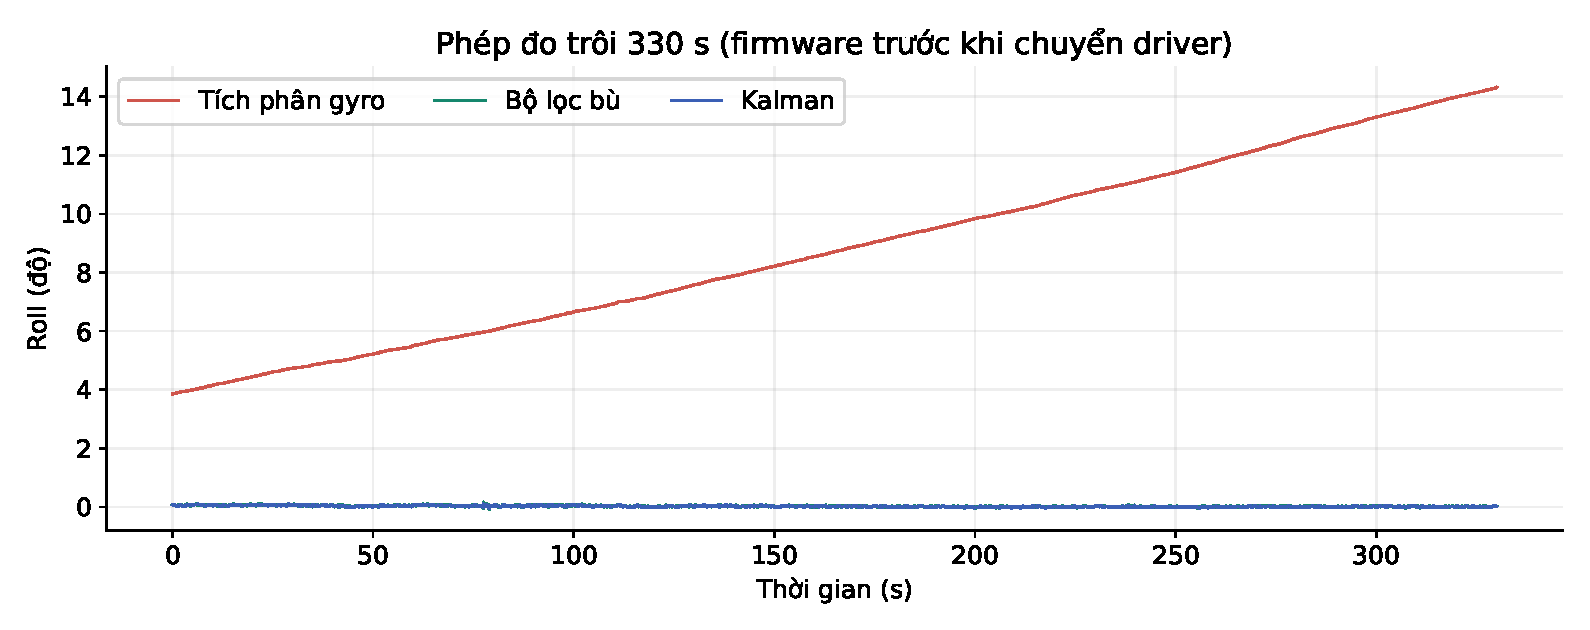
\includegraphics[width=\textwidth]{drift_330s.pdf}
\caption{Trôi Roll trong 330 giây theo dữ liệu \texttt{drift5p.csv}.}\label{fig:drift}
\end{figure}

\begin{table}[htbp]\centering\fontsize{12}{17}\selectfont
\caption{So sánh độ trôi và dao động trong 330 giây.}\label{tab:drift}
\begin{tabular}{|L{43mm}|C{34mm}|C{29mm}|C{27mm}|}
\hline Phương pháp & Độ lệch đầu--cuối & Biên độ & Độ lệch chuẩn\\ \hline
Gyro-only Roll & $+10{,}46\degree$ & $10{,}5\degree$ & $3{,}03\degree$\\ \hline
Gyro-only Pitch & $-3{,}82\degree$ & $3{,}8\degree$ & $1{,}09\degree$\\ \hline
Bộ lọc bù Roll & Gần $0\degree$ & $0{,}25\degree$ & $0{,}025\degree$\\ \hline
Kalman Roll & Gần $0\degree$ & $0{,}15\degree$ & $0{,}024\degree$\\ \hline
\hline
\end{tabular}
\end{table}

Kết quả 330~s hỗ trợ nhận xét rằng hai bộ lọc không trôi đáng kể trong điều kiện đặt yên của phép đo cũ. Nó không chứng minh mọi điều kiện nhiệt độ hay rung đều không trôi; bản tích hợp cuối cần một log lặp lại với cùng quy trình.

\section{Phép đo bàn servo trên bản tích hợp cuối}
Servo được ra lệnh theo chuỗi $0\to30\to60\to90\to60\to30\to0\degree$, di chuyển với tốc độ đặt khoảng $1\degree/80$~ms. Bảng~\ref{tab:servo_final} dùng trung bình 100 mẫu ổn định cuối mỗi nấc và lấy nấc đầu làm mốc tương đối. Dây đánh dấu chỉ kiểm tra vị trí quay về $0\degree$; các giá trị $30/60/90\degree$ là góc lệnh servo, không phải số đo từ thước góc độc lập.

\begin{table}[htbp]\centering\fontsize{12}{17}\selectfont
\caption{Góc Kalman Roll tương đối trong phép đo servo ngày 20/10/2026.}\label{tab:servo_final}
\begin{tabular}{|C{25mm}|C{34mm}|C{34mm}|C{30mm}|}
\hline Góc lệnh & Chiều đi ($\degree$) & Chiều về ($\degree$) & Độ lệch chuẩn ($\degree$)\\ \hline
$0\degree$ & $0{,}00$ & $-0{,}16$ & $0{,}012$--$0{,}022$\\ \hline
$30\degree$ & $24{,}81$ & $28{,}36$ & $0{,}016$--$0{,}022$\\ \hline
$60\degree$ & $51{,}77$ & $52{,}91$ & $0{,}013$\\ \hline
$90\degree$ & $79{,}82$ & -- & $0{,}033$\\ \hline
\hline
\end{tabular}
\end{table}

Sai khác hai chiều tại lệnh $60\degree$ là $1{,}16\degree$ và tại $30\degree$ là $3{,}55\degree$, thể hiện độ rơ/cản cơ khí của cơ cấu. Góc quay về mốc dây lệch $-0{,}16\degree$, cho thấy khả năng lặp lại quanh điểm gốc trong lần thử này. Tỷ lệ giữa góc Kalman và góc lệnh không đạt một, nên dữ liệu không hỗ trợ tuyên bố ``sai số Kalman dưới $1\degree$''; nó chủ yếu chứng minh luồng đo tích hợp, độ ổn định tại nấc và ảnh hưởng của bàn servo.

\section{So sánh bốn phương pháp khi xoay tay}
Hình~\ref{fig:dynamic} dùng 1\,503 mẫu trong khoảng 30~s. Đây là phép thí nghiệm chung cho góc gia tốc, tích phân gyro, bộ lọc bù và Kalman. Đường gyro tích lũy lệch rõ sau quá trình xoay, còn hai đường hợp nhất cảm biến bám xu hướng của góc gia tốc và ít nhiễu hơn. Vì phép xoay tay không có góc tham chiếu độc lập, hình chỉ cho phép đánh giá xu hướng và độ trôi tương đối; không dùng để kết luận MAE hoặc ngưỡng sai số tĩnh $<1\degree$.

\begin{figure}[htbp]\centering
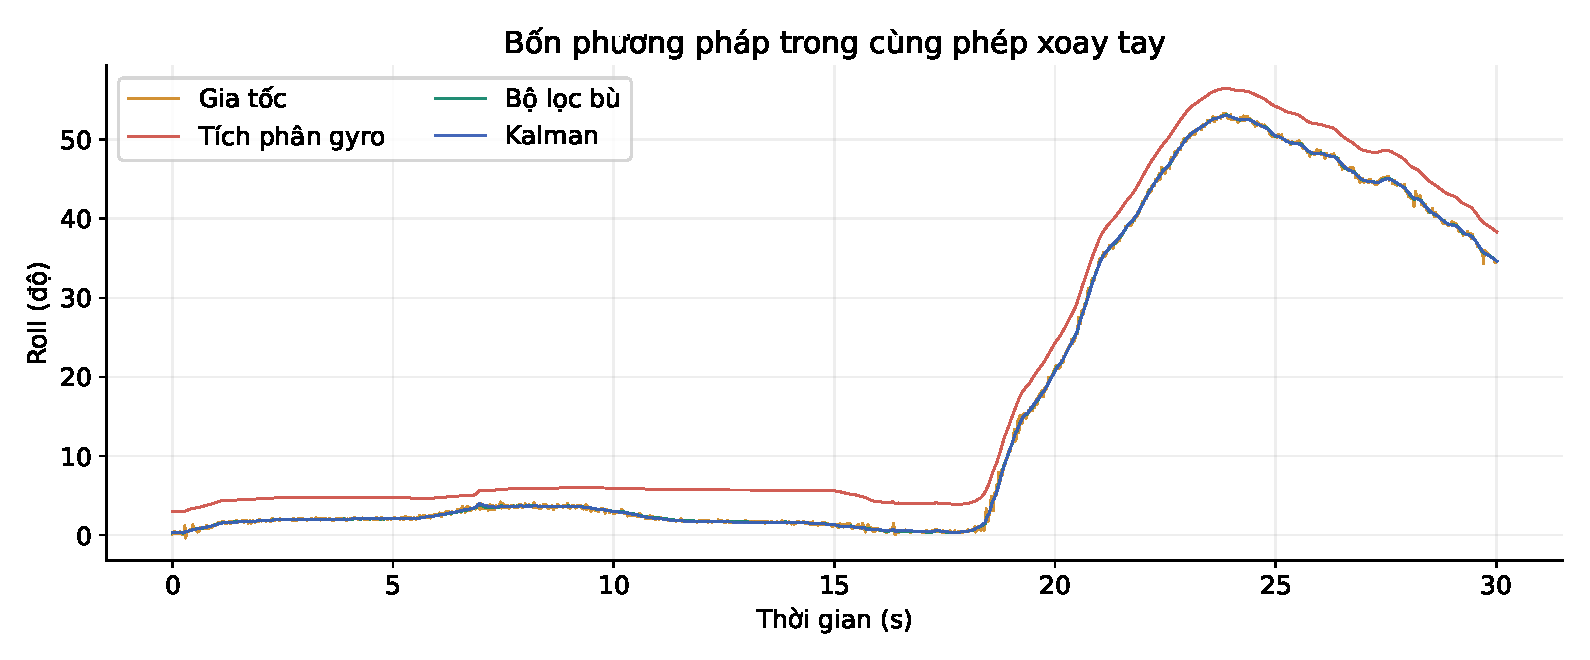
\includegraphics[width=\textwidth]{bon_phuong_phap_dong.pdf}
\caption{Bốn phương pháp trên cùng phép xoay tay; chưa có góc chuẩn độc lập.}\label{fig:dynamic}
\end{figure}

\section{Đáp ứng khi rung}
Trong file \texttt{vibration.csv}, đoạn 10~s đầu gần như đứng yên và đoạn 10--20~s có tác động rung. Độ lệch chuẩn của góc gia tốc tăng từ $0{,}076\degree$ lên $1{,}102\degree$; bộ lọc bù ở đoạn rung là $0{,}101\degree$, còn Kalman là $0{,}064\degree$. Hình~\ref{fig:vibration} cho thấy các xung nhiễu của gia tốc được làm dịu khi kết hợp với gyro. Đoạn cuối của file vẫn còn rung, nên không dùng làm khoảng phục hồi sau rung.

\begin{figure}[htbp]\centering
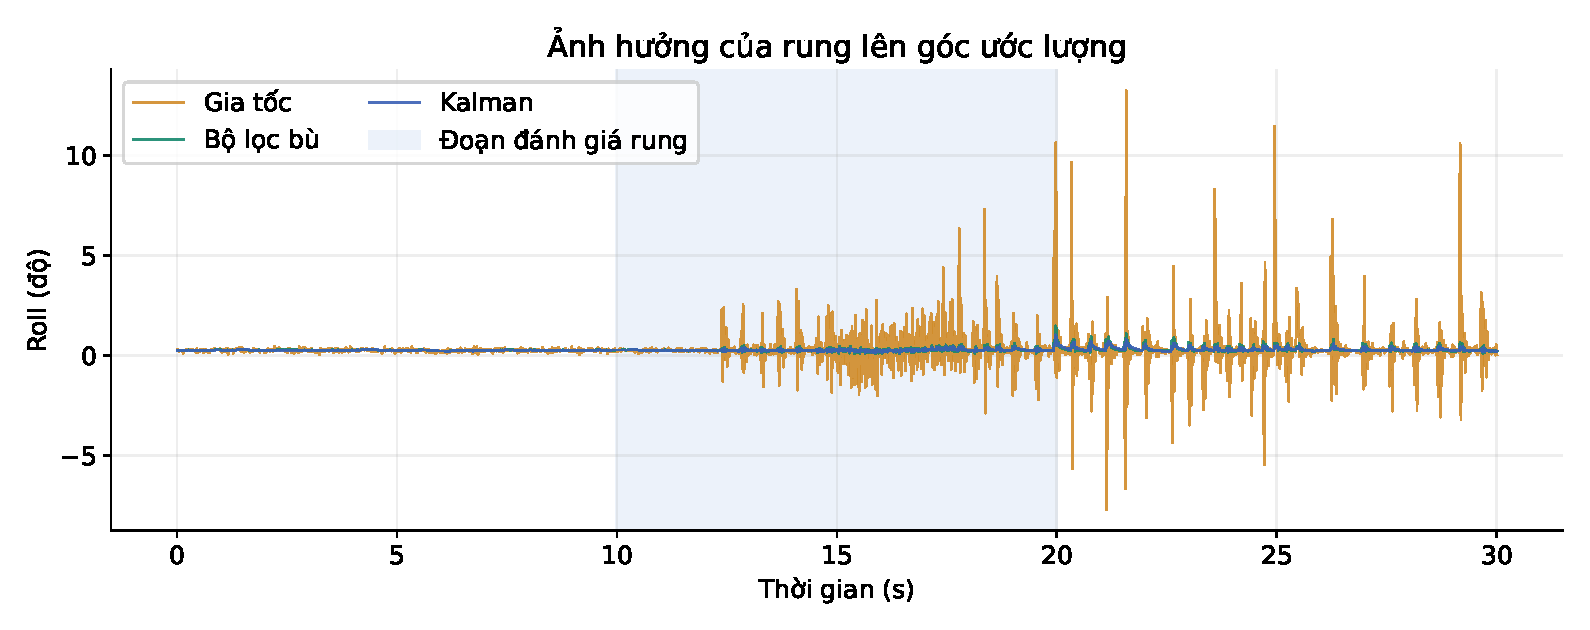
\includegraphics[width=\textwidth]{rung.pdf}
\caption{Góc Roll trong phép đo rung, vùng tô là đoạn 10--20 giây.}\label{fig:vibration}
\end{figure}

\section{Tinh chỉnh tham số và dữ liệu so sánh lịch sử}
Quét $\alpha$ ngoại tuyến trên đoạn tĩnh cho điểm nhỏ nhất của chỉ số RMSE quanh trung bình gia tốc tại $\alpha=0{,}98$ trong các giá trị đã thử. Vì mốc so sánh là chính tín hiệu gia tốc, chỉ số này phản ánh độ ổn định tương đối, không phải sai số so với góc thật.

\begin{table}[htbp]\centering\fontsize{12}{17}\selectfont
\caption{Kết quả quét hệ số bộ lọc bù trên dữ liệu tĩnh.}\label{tab:alpha}
\begin{tabular}{|C{20mm}|*{6}{C{17mm}|}}
\hline $\alpha$ & 0,90 & 0,95 & 0,97 & 0,98 & 0,99 & 0,995\\ \hline
RMSE ($\degree$) & 0,0173 & 0,0131 & 0,0114 & \textbf{0,0109} & 0,0127 & 0,0179\\ \hline
\hline
\end{tabular}
\end{table}

Trong phép đo 330~s của firmware cũ, chênh lệch lớn nhất giữa góc Kalman float và bản Q16.16 một phần là $0{,}01\degree$ cho Roll/Pitch; một file tích hợp cũ ghi $0{,}00081\degree$. Đây là dữ liệu lịch sử về hai triển khai, không phải sai số so với góc chuẩn. Firmware hiện tại đã bỏ bản Kalman fixed và chỉ giữ bản float.

\section{Thời gian thực thi và jitter}
File tích hợp lịch sử có 1\,728 gói hợp lệ, không có frame CRC lỗi. Chu kỳ mẫu có trung bình $1\,997{,}58~\mu\mathrm{s}$, độ lệch chuẩn $2{,}04~\mu\mathrm{s}$ và khoảng $1\,993$--$2\,002~\mu\mathrm{s}$, phù hợp mục tiêu 500~Hz. Trường \texttt{exec\_us} có trung bình $677{,}72~\mu\mathrm{s}$, khoảng $668$--$681~\mu\mathrm{s}$, thấp hơn chu kỳ 2~ms. Mốc đo \texttt{exec\_us} kết thúc sau cập nhật các bộ lọc và trước phần từ kế, đóng gói telemetry và đẩy OLED; do đó \texttt{dt\_us} mới là bằng chứng bao quát hơn cho lịch lấy mẫu khi các tác vụ nền cùng hoạt động.

\section{Màn OLED và giao diện giám sát}
OLED 128$\times$64 hiển thị bốn ô \texttt{ROLL}, \texttt{PITCH}, \texttt{YAW} và \texttt{REF}, mỗi góc có hai chữ số thập phân. Framebuffer 1~KB được gửi từng page; tốc độ 10 page/s làm một khung hoàn chỉnh mất khoảng 0,8~s nhưng hạn chế thời gian chiếm bus I2C. Giao diện web hiện giải mã packet 77 byte, CRC-8, biểu đồ, mô hình 3D, thống kê và xuất CSV. Web Serial hoạt động trên Chrome/Edge và Firefox 151+ bản desktop; trang phải chạy trên \texttt{localhost} hoặc HTTPS. Với Firefox, extension WebSerial cũ và sandbox của gói Snap có thể gây xung đột hoặc che thiết bị serial.

\needspace{7\baselineskip}
\section{Đối chiếu yêu cầu đề K03}
\begin{longtable}{|L{44mm}|L{27mm}|L{64mm}|}
\caption{Trạng thái bằng chứng đối với các yêu cầu chính.}\label{tab:requirements}\\
\hline Yêu cầu & Trạng thái & Căn cứ và việc còn cần làm\\ \hline
\endfirsthead
\hline Yêu cầu & Trạng thái & Căn cứ và việc còn cần làm\\ \hline
\endhead
Tự viết bốn phương pháp tính góc & Có mã, có log & Module C riêng; Hình~\ref{fig:dynamic} dùng cùng một phép đo.\\ \hline
500~Hz, hiệu chuẩn, ngắt Data Ready & Đã đo trên bản cũ & 1\,728 gói; $dt=1\,997{,}58\pm2{,}04~\mu\mathrm{s}$, cần đo lại trên bản hiện tại.\\ \hline
Kalman float & Đã tích hợp & Bản hiện tại chỉ dùng một Kalman hai trạng thái dạng float; số đo fixed thuộc bản cũ.\\ \hline
Kalman không trôi sau 5 phút & Có bằng chứng bản cũ & Log 330~s, Hình~\ref{fig:drift}; đo lặp lại trên bản cuối.\\ \hline
Sai số tĩnh Kalman dưới $1\degree$ & Chưa kết luận & Cần góc chuẩn độc lập ở nhiều nấc servo, MAE/RMSE và bất định chuẩn.\\ \hline
Độ trễ và đáp ứng bước & Có chuỗi nấc tĩnh & Đã có $0\to90\to0\degree$; chưa có góc thật theo thời gian để tách trễ cơ khí và thuật toán.\\ \hline
OLED hoặc LED 7 đoạn & Đã tích hợp & Bố cục bốn ô đã có trong firmware; cần ảnh/video màn OLED thật cho hồ sơ nộp.\\ \hline
Đồ thị realtime và mô hình 3D & Đã có Web Serial & Đã nối bộ giải mã binary/CRC; cần quay demo trực tiếp với mạch.\\ \hline
Sơ đồ, báo cáo, video 3--5 phút & Có tài liệu thiết kế & Đã có sơ đồ nối chân, lưu đồ và số liệu; ảnh mạch và video là minh chứng riêng.\\ \hline
\hline
\end{longtable}

\section{Nhận xét và giới hạn}
Kết quả tĩnh và trôi dài hạn cho thấy cả bộ lọc bù lẫn Kalman đều khai thác được mốc trọng lực để hạn chế tích lũy sai số của gyro. Ở trạng thái tĩnh, chênh lệch độ lệch chuẩn giữa hai bộ lọc nhỏ. Trong đoạn rung đã khảo sát, Kalman cho độ lệch chuẩn thấp hơn bộ lọc bù, phù hợp với ưu điểm của việc hiệu chỉnh trạng thái bằng mô hình và hiệp phương sai.

Các phép đo xoay tay và gõ bàn chưa tạo ra một kích thích có biên độ, tần số và góc chuẩn được kiểm soát. Do đó, kết quả phản ánh hành vi của hệ thống trong các điều kiện đã ghi, chưa cho phép suy rộng thành độ chính xác tuyệt đối hoặc đáp ứng tần số của toàn bộ hệ thống. Bàn servo cần được đối chiếu với một chuẩn góc độc lập trước khi dùng để kiểm tra ngưỡng sai số dưới $1\degree$.

Về triển khai, số liệu tích hợp xác nhận nhịp lấy mẫu và thời gian phần lõi, nhưng chưa đo benchmark từng hàm. Phần Yaw hiện là mở rộng; từ kế đặt gần servo có thể chịu nhiễu từ, vì vậy cần hiệu chuẩn hard/soft iron, bù nghiêng và mốc hướng độc lập trước khi chấm độ chính xác Yaw.

\section{Đọc kết quả theo cùng điều kiện thí nghiệm}
Các hình trong Chương~3 có ích khi được đọc cùng cấu hình phép đo. Đường đứng yên 330~s chứng minh hành vi dài hạn trong một lần đặt board yên. Đường xoay tay chứng minh hành vi khi góc thay đổi nhưng không có chuẩn góc độc lập. Đường rung chứng minh độ suy giảm dao động của đầu ra trong điều kiện kích thích đã ghi. Ba phép thử bổ sung cho nhau; không phép thử riêng lẻ nào đủ để khẳng định mọi tiêu chí của đề K03. Cách đối chiếu hợp lý là nêu biến quan sát, điều kiện tác động, chỉ số và giới hạn của từng phép đo.

\subsection{Phép đo đứng yên và trôi dài hạn}
Trong file \,\texttt{drift5p.csv}\, có 16\,519 mẫu log ở khoảng 50~Hz, trải khoảng 330~s. Gyro-only Roll đổi khoảng $+10{,}46\degree$, còn hai đường hợp nhất giữ quanh một mốc. Kết quả này phù hợp cơ chế tích lũy bias của tích phân và cơ chế kéo về mốc trọng lực của CF/Kalman. Nếu chỉ trừ một mẫu đầu và một mẫu cuối, số đo rất nhạy với ngoại lệ; nên so trung bình cửa sổ đầu và cuối, đồng thời báo độ lệch chuẩn và khoảng dao động của từng cửa sổ. Bảng~\ref{tab:drift} là tóm tắt từ nhật ký cũ, chưa ghi bất định qua nhiều lần lặp.

Một đường ``gần như không trôi'' trong 330~s không có nghĩa bias tuyệt đối bằng không. Nếu mặt bàn nghiêng hoặc hiệu chuẩn gia tốc còn sai, bộ lọc có thể hội tụ về một góc sai nhưng ổn định. Vì vậy, kết luận được hỗ trợ bởi phép đo này là độ ổn định dài hạn trong một điều kiện đặt yên, không phải độ chính xác tuyệt đối. Việc có cả biên độ và độ lệch chuẩn giúp tách một xung ngoại lệ ngắn ra khỏi dao động thường xuyên; nên xem đồ thị gốc để kiểm tra có va chạm nhẹ trong quá trình đo hay không.

\subsection{Phép đo động xoay tay}
File \,\texttt{dynamic.csv}\, có khoảng 1\,503 hàng trong 30~s. Khi xoay, gia tốc cho mốc góc tức thời nhưng nhiễu, gyro-only cho đường liên tục nhưng có thể lệch mốc, CF/Kalman kết hợp hai nguồn. Nhật ký ghi chênh lệch gyro-only khoảng $35{,}4\degree$ trên phép xoay liên tục. Đại lượng này cần được hiểu theo cách tạo đồ thị và mốc khởi tạo; không được gọi là sai số độ chính xác nếu chưa đo góc thật ở từng thời điểm. Đồ thị chung vẫn rất hữu ích để minh họa bốn đặc tính và phát hiện sai dấu hoặc sai trục khi tích hợp.

Một cách đánh giá có kiểm soát hơn là đặt board trên bàn quay với các nấc góc biết trước và một bước có thời điểm lệnh xác định. Lúc đó, ở mỗi nấc có thể so bias tĩnh; quanh bước có thể so thời gian đáp ứng. Cùng một chuỗi dữ liệu phải được đưa vào cả bốn phương pháp, vì thay đổi tốc độ xoay tay giữa các lần đo làm mất cơ sở so sánh. Khi chưa có bàn quay được hiệu chuẩn, nên giữ phép xoay tay như minh họa định tính và không dựng bảng MAE từ nó.

\subsection{Phép đo rung và giới hạn diễn giải}
Ở đoạn rung 10--20~s của file \,\texttt{vibration.csv}\,, độ lệch chuẩn góc gia tốc khoảng $1{,}102\degree$, CF khoảng $0{,}101\degree$, Kalman khoảng $0{,}064\degree$. Tỷ số theo độ lệch chuẩn cho thấy tín hiệu Kalman dao động ít hơn góc gia tốc trong đoạn đó. Tuy nhiên, lực gõ bàn không được định lượng theo biên độ hoặc phổ tần, và 10~s cuối vẫn có rung. Vì vậy, phép thử không thể cho một hàm truyền rung hay chứng minh thuật toán luôn chính xác hơn CF trong mọi loại chuyển động.

Để lặp lại phép rung, cần giữ cùng cách gá, cùng khoảng cách tới nguồn rung, cùng dải tần và thời gian tác động. Nếu có động cơ rung, nên ghi điện áp và vị trí của nó. Nếu không có, mô tả cách gõ và số lần gõ vẫn tốt hơn bỏ trống điều kiện. Khi phân tích, lấy một đoạn nền đứng yên và đoạn rung có cùng độ dài, rồi so cả độ lệch chuẩn, phần trăm mẫu vượt ngưỡng và độ trễ hồi về sau rung. Chỉ nên tính đoạn hồi phục nếu log thật có khoảng dừng rung rõ ràng.

\section{Đánh giá tham số và quan hệ giữa các chỉ số}
\subsection{Hệ số bộ lọc bù}
Bảng~\ref{tab:alpha} cho thấy giá trị RMSE nhỏ nhất trong những $\alpha$ đã quét là 0,98. Mốc so sánh của lần quét là trung bình góc gia tốc trên đoạn tĩnh. Do đó, bảng xếp hạng này ưu tiên tín hiệu ổn định quanh một trung bình nội bộ; nó không kiểm tra độ trễ STEP hay sai số theo góc thật. Nếu chọn $\alpha$ chỉ theo độ mịn tĩnh, hệ số quá cao có thể làm kết quả chậm sau một bước quay. Lần đo tiếp theo nên đánh giá đa tiêu chí: sai số tại các nấc có chuẩn, độ lệch chuẩn khi đứng yên, thời gian xác lập sau bước và nhiễu khi rung.

Với Kalman, $Q$ và $R$ cũng có quan hệ đánh đổi tương tự nhưng trong cấu trúc có ước lượng bias. Thử một bộ tham số trên dữ liệu đã dùng để chọn chính bộ đó có nguy cơ cho kết quả tốt giả tạo. Nên chia dữ liệu thành tập chọn tham số và tập kiểm tra riêng, hoặc ít nhất dùng hai lần đo độc lập với cùng quy trình. Mọi bộ tham số được công bố phải khớp với mã firmware tạo ra số liệu; nếu chạy replay Python mà firmware dùng số khác, cần ghi rõ đây là thử ngoại tuyến.

\subsection{Độ chính xác, độ mịn và hiệu quả chống trôi}
Ba câu hỏi định lượng phải được trả lời bằng ba chỉ số khác nhau. ``Góc có đúng không?'' cần chuẩn độc lập và MAE/RMSE/bias. ``Đường có mượt không?'' cần độ lệch chuẩn hoặc phổ nhiễu trong một đoạn đứng yên. ``Đường có trôi không?'' cần so đầu--cuối trên thời gian đủ dài. Một phương pháp có thể cho độ lệch chuẩn rất nhỏ vì làm trơn mạnh, nhưng đồng thời chậm hoặc lệch mốc. Khi báo cáo tổng hợp, nên đặt các chỉ số cạnh nhau cho từng phương pháp và giải thích lý do ưu tiên theo ứng dụng.

Nếu sử dụng góc lệnh servo làm chuẩn tạm thời, các chỉ số nên được ghi là ``sai lệch so với góc lệnh'', không gọi là ``sai số tuyệt đối''. Sau khi hiệu chuẩn servo, báo thêm bất định của chuẩn và sai khác theo chiều quay. Chỉ khi bất định đủ nhỏ và kết quả lặp lại qua nhiều nấc mới có cơ sở xác nhận điều kiện $<1\degree$ của đề. Một nấc $0\degree$ không đại diện cho dải $\pm60\degree$, vì sai lệch scale và sai trục có thể tăng theo góc.

\section{Đánh giá tính thời gian thực}
\subsection{Ngân sách 2 ms cho một mẫu}
Ở 500~Hz, tổng công việc bắt buộc cho một mẫu phải hoàn thành trước khi có mẫu kế tiếp, tức dưới 2~ms trong điều kiện bình thường. Log tích hợp cuối có \texttt{exec\_us} trung bình $677{,}72~\mu\mathrm{s}$, cực đại $681~\mu\mathrm{s}$ và chu kỳ mẫu $1\,997{,}58\pm2{,}04~\mu\mathrm{s}$. Kết quả xác nhận phần lõi còn khoảng dự phòng và lịch lấy mẫu được duy trì trong lần chạy 1\,728 frame. Vì điểm kết thúc \texttt{exec\_us} nằm trước từ kế, telemetry và OLED, chi phí riêng từng khối vẫn cần đo nếu muốn tối ưu sâu hơn.

Đo bằng DWT cần đặt điểm bắt đầu và kết thúc nhất quán. Nếu đồng hồ bắt đầu ngay trước đọc I2C và dừng sau cập nhật Kalman, số đo không bao gồm OLED và gửi gói. Nếu điểm kết thúc sau tất cả tác vụ trong vòng lặp, số đo phản ánh tổng tải nhưng khó quy lỗi cho một khối. Nên đo cả hai, và trình bày sơ đồ phạm vi đo. Các bảng hiệu năng phải ghi compiler optimization, clock, baud, trạng thái các module và số mẫu đo. Điều này đặc biệt quan trọng khi so sánh float và Q16.16 một phần.

\subsection{Jitter và độ trễ đầu cuối}
Jitter chu kỳ của log tích hợp có độ lệch chuẩn $2{,}04~\mu\mathrm{s}$, gần số đo cũ $1{,}84~\mu\mathrm{s}$. Độ trễ đầu cuối từ lệnh servo tới đồ thị PC gồm thêm thời gian chờ PWM 20~ms, động học servo, lấy mẫu tối đa 2~ms, xử lý, chờ telemetry tối đa 20~ms và trễ truyền/hiển thị. Do các thành phần này khác nhau, jitter lấy mẫu nhỏ không có nghĩa đồ thị PC đáp ứng tức thời. Khi công bố độ trễ, phải nói rõ đo từ mốc nào tới mốc nào.

Ở nhịp telemetry 50~Hz, một điểm xuất hiện cách nhau khoảng 20~ms. Nếu ước lượng độ trễ bằng thời điểm vượt ngưỡng trên các điểm đó, bất định do lượng tử hóa thời gian đã ở cỡ một chu kỳ hiển thị. Nội suy đồ thị có thể làm đường mượt nhưng không tạo thêm thông tin thời gian thực. Muốn đo độ trễ ở mức mili giây, cần log dấu thời gian nội bộ cho sự kiện đổi ref và từng mẫu 500~Hz, hoặc đo đồng thời chân PWM và một tín hiệu phản ánh góc thật bằng thiết bị ngoài.

\section{Giới hạn của phiên bản hiện tại và thứ tự hoàn thiện}
Mã nguồn hiện tại tích hợp driver MPU6500 mức thanh ghi, CF, Kalman float/fixed, OLED, từ kế tùy chọn và gói telemetry; servo của phép đo cuối do ESP32-S3 điều khiển độc lập. Log mới đủ chứng minh hoạt động tích hợp, nhịp lấy mẫu và độ nhất quán số học. Bảng kết quả cũ vẫn có giá trị giải thích drift/rung, nhưng được giữ nhãn phiên bản lịch sử.

Các việc còn lại theo thứ tự ưu tiên là: chụp ảnh OLED và toàn mạch; quay demo Web Serial/3D; đo góc bằng chuẩn độc lập khi có dụng cụ; benchmark từng hàm và bộ nhớ; hiệu chuẩn/bù nghiêng từ kế. Sau mỗi phép thử cần ghi phiên bản và file log để không trộn bằng chứng giữa các cấu hình.

Ảnh sản phẩm trong mục tiếp theo được để trống có chủ đích. Khi chụp, nên thấy đủ dây nguồn, tên chân quan trọng, hướng trục cảm biến và cơ cấu gá; không dùng ảnh đồ họa mô phỏng để thay thế bằng chứng phần cứng. Ảnh màn OLED cần chụp cùng một tư thế có góc tham chiếu; ảnh màn PC cần thấy đồ thị bốn phương pháp và dấu thời gian. Mỗi ảnh nên ghi ngày, cấu hình chạy và chú thích ngắn về điều nó chứng minh.


\section{Ảnh sản phẩm và bố trí thí nghiệm thực tế}
Những khung dưới đây dành cho ảnh chụp của chính nhóm sau khi hoàn tất lắp ráp. Trước khi nộp, thay từng khung bằng \,\texttt{\textbackslash includegraphics}\, đúng ảnh tương ứng và giữ chú thích theo nội dung đã kiểm chứng. Không đưa ảnh của bản thử servo đơn lẻ vào mục ``mạch tích hợp'' nếu các module còn lại chưa cùng hoạt động. Ảnh chỉ chứng minh cấu hình vật lý tại thời điểm chụp. Kết luận về độ chính xác và tốc độ phải dựa trên file log và bảng phân tích từ đúng lần chạy đó.

\ChoAnhThucTe{Mặt trên của board, vị trí STM32, MPU6500, OLED và từ kế.}{Toàn cảnh sản phẩm hoàn thiện nhìn từ mặt trên.}

\ChoAnhThucTe{Mặt bên hoặc phía dưới cho thấy dây 3,3 V, dây 5 V, mass chung, PA0, PB6/PB7, UART và ESP32-S3 GPIO21.}{Đấu nối và phân chia nguồn trên mô hình thực tế.}

\ChoAnhThucTe{Cơ cấu servo, vị trí cố định thân servo, còi, hướng trục MPU6500 và thước góc độc lập.}{Bàn quay servo dùng trong phép thử Roll.}

\ChoAnhThucTe{Màn OLED trong lúc mạch chạy; chụp cùng trạng thái góc và dấu thời gian của phép thử.}{Góc hiển thị trên màn OLED của mạch.}

\ChoAnhThucTe{Màn máy tính hiển thị bốn đường góc cùng một lần đo và mô hình 3D nếu đã kết nối với bản firmware cuối.}{Giao diện giám sát và đối chiếu dữ liệu trên PC.}

\ChoAnhThucTe{Bố trí phép đo STATIC hoặc STEP với thiết bị đo góc độc lập và toàn bộ nguồn cấp.}{Bố trí thí nghiệm đối chứng trên mạch hoàn chỉnh.}

\subsection{Thông tin cần ghi kèm ảnh}
Với ảnh toàn cảnh, cần ghi ngày chụp, nguồn điện sử dụng và phiên bản firmware đang chạy. Với ảnh sơ đồ dây thực tế, chú thích nên chỉ rõ chân PA0 nhận ngắt từ MPU6500, PB6/PB7 là bus I2C, PA9/PA10 dành cho UART và ESP32-S3 GPIO21 phát PWM servo. Nếu dùng phương án servo nội STM32 thì mới ghi PA1/TIM2\_CH2. Các nhãn này phải đặt theo dây thật, không chỉ theo sơ đồ dự kiến.

Với ảnh bàn servo, cần đặt mốc $0\degree$ và hướng dương trên cùng mặt ảnh, để người đọc hiểu vì sao góc ref được so với Roll. Ảnh ở hai góc khác nhau giúp chứng minh cơ cấu thật sự quay và cách gá không cản dây. Với ảnh OLED, cần tránh chụp khi màn hình đang đổi số hoặc bị lóa; có thể ghi góc hiển thị và góc tham chiếu ngay trong chú thích. Ảnh màn PC cần thấy tên các đường, trục thời gian, đơn vị độ và nguồn dữ liệu. Nếu ảnh 3D được chụp từ file cũ trong khi board chạy firmware mới, phải ghi rõ trạng thái đó; ảnh demo cuối cần dùng đúng nguồn telemetry của bản tích hợp.

Khi chèn ảnh vào LaTeX, giữ tỷ lệ gốc của ảnh, chỉ đặt một giới hạn chiều rộng và chiều cao. Có thể dùng \texttt{width=0.86\textbackslash textwidth} và \texttt{keepaspectratio}; nếu ảnh dọc, giới hạn thêm chiều cao để chú thích không bị đẩy sang trang sau. Không phóng ảnh mờ hoặc nén đến mức không đọc được nhãn chân, số trên OLED và trục đồ thị. Nếu một ảnh không thể chụp được, cần bỏ khung tương ứng khỏi bản nộp và diễn giải giới hạn bằng văn bản; không để lại khung trống trong bản cuối.


\chapter{QUY TRÌNH KIỂM CHỨNG BẢN TÍCH HỢP}

\section{Mục đích và trạng thái bằng chứng}
Chương này quy định cách bổ sung các bằng chứng còn thiếu sau phép đo tích hợp ngày 20/10/2026. File log hiện tại xác nhận đường dữ liệu, nhịp 500~Hz, chuỗi servo và độ ổn định tại các nấc; các tiêu chí độ chính xác tuyệt đối, độ trễ thuật toán và Yaw vẫn cần chuẩn đo độc lập. Ảnh, video và số liệu phải xuất phát từ cùng cấu hình phần cứng và firmware.

Mỗi lần thử cần một mã nhận dạng duy nhất gồm ngày giờ, mã commit, cấu hình biên dịch và mã file CSV. Trong sổ đo nên ghi board, nguồn cấp, baud UART, trạng thái OLED/từ kế, cách gá cảm biến, nhiệt độ môi trường nếu có, giá trị $\alpha,Q,R$, thời gian hiệu chuẩn gyro và tên kịch bản servo. Khi một điều kiện thay đổi, cần tạo lần đo mới. Việc ghi này giúp phân biệt sai số do thuật toán với sai số do mạch, servo và môi trường.

\section{Kiểm tra chức năng từng tầng}
\subsection{Nguồn, clock và cảm biến}
Trước tiên đo điện áp 3,3~V tại module MPU và OLED, điện áp 5~V tại servo khi đứng yên và khi chuyển nấc. Kiểm tra mass chung. Sau đó đọc các thanh ghi clock và xác nhận tần số hệ thống 72~MHz. Trên I2C, xác nhận địa chỉ MPU 0x68 hoặc 0x69 tùy AD0 và WHO\_AM\_I bằng 0x70. Một log khởi động nên chứa giá trị đọc, địa chỉ tìm thấy, cấu hình DLPF và bộ chia mẫu. Khi đọc burst 14 byte, đặt board phẳng để xem $a_z$ gần $1g$ và ba vận tốc góc sau hiệu chuẩn gần không. Đây là phép kiểm hợp lý, chưa phải hiệu chuẩn góc chuẩn.

Để kiểm EXTI, đếm số sự kiện Data Ready trong một khoảng 30~s và so với xấp xỉ 15\,000 sự kiện danh định. Đồng thời đếm số lần vòng lặp xử lý mẫu và số timeout I2C. Nếu đếm ngắt tăng đúng nhưng số mẫu xử lý thấp, vòng lặp hoặc cờ Boolean đã bỏ mẫu. Nếu cả hai thấp, cần kiểm cấu hình INT của MPU và PA0. Việc nêu cả số lần thành công lẫn số lần thất bại hữu ích hơn chỉ ghi ``500 Hz'' trong bảng cấu hình.

\subsection{Từng thuật toán và đầu ra}
Với board đứng yên, ghi đồng thời góc gia tốc, gyro-only, CF và Kalman float trong 30~s. Kiểm tra mỗi giá trị hữu hạn, không nhảy bất thường và dấu góc đúng khi nghiêng chậm từng trục. Sau đó thực hiện một lần quay thuận rồi quay ngược về vị trí ban đầu; xem đường gyro-only có lệch mốc và CF/Kalman có trở về mốc hay không. Cần lưu cả dữ liệu thô sáu trục để khi đường góc sai có thể truy lại lỗi đổi đơn vị hoặc lỗi thứ tự byte.

OLED phải hiển thị số đọc có cùng dấu và cùng đơn vị với telemetry. Nếu OLED cập nhật chậm hơn, điều đó cần được mô tả như khác biệt tần suất hiển thị. Từ kế được kiểm riêng bằng một vòng xoay ngang và phép nghiêng tại hướng cố định; kết quả Yaw chỉ được chấm định lượng khi đã có hiệu chuẩn từ trường và mốc hướng độc lập. Với phần mềm PC, kiểm CRC và số gói mất trước khi mở đồ thị realtime hoặc mô hình 3D.

\section{Thiết kế bộ phép thử cuối}
\begin{table}[htbp]\centering\fontsize{11}{15}\selectfont
\caption{Bộ phép thử cần chạy trên đúng phiên bản firmware tích hợp.}\label{tab:final_tests}
\begin{tabular}{|L{27mm}|L{52mm}|L{54mm}|}\hline
Phép thử & Dữ liệu cần thu & Kết quả cần xuất\\\hline
STATIC & Bảy nấc servo, góc chuẩn độc lập, bốn phương pháp & MAE, RMSE, bias, độ lệch chuẩn theo từng nấc\\\hline
STEP & Dấu thời gian lệnh, góc thật và góc ước lượng & Trễ, thời gian xác lập, vọt lố có định nghĩa rõ\\\hline
DRIFT & Ít nhất 330~s giữ yên, mẫu đầu/cuối & Độ trôi trung bình cửa sổ, biên độ, số mẫu mất\\\hline
RUNG & Đoạn nền và đoạn tác động có mốc thời gian & Độ lệch chuẩn, ngoại lệ, điều kiện kích thích\\\hline
TẢI ĐẦY ĐỦ & OLED, từ kế, servo, telemetry cùng chạy & Phân bố $\Delta t$, thời gian xử lý, số chu kỳ quá 2~ms\\\hline
\end{tabular}
\end{table}

Với STATIC, nên chạy ít nhất hai vòng quét theo hai chiều để đánh giá độ rơ servo. Mỗi nấc phải có thời gian bỏ chuyển động và thời gian lấy trung bình được ghi rõ. Nếu dùng cùng một thước góc cho các nấc, nên đọc lặp lại hoặc chụp ảnh thước cùng board để kiểm sai số đọc. Kết quả chính cần trình bày theo từng nấc trước khi tính một chỉ số gộp; chỉ số gộp có thể che một góc biên kém hơn các góc giữa.

Với DRIFT, thời gian ít nhất 330~s cho phép so với yêu cầu ``trên 5 phút''. Cần xác nhận mạch và servo không bị chạm trong khoảng này. Chọn trước kích thước cửa sổ đầu và cuối, ví dụ 10~s, để tránh chọn cửa sổ sau khi nhìn thấy kết quả. Nếu có thay đổi nhiệt độ đáng kể hoặc nguồn servo dao động, ghi chúng như điều kiện ảnh hưởng. Phép này nên lặp lại sau một lần tắt/bật để xem độ tái lập.

Với STEP, phải tránh gọi góc lệnh là góc thật. Nếu không có cảm biến vị trí độc lập theo thời gian, có thể báo đường đáp ứng so với lệnh như phép minh họa, kèm giới hạn. Nếu có góc thật, quy trình xác định mức đầu, mức cuối, thời điểm vượt 10\%, 50\% và 90\% biên độ nên giống nhau cho cả bốn phương pháp. Độ trễ của thuật toán là hiệu thời điểm giữa góc thật và góc ước lượng, với dấu thời gian đã đồng bộ.

\section{Mẫu bảng kết quả cần điền sau phép đo}
\begin{table}[H]\centering\fontsize{11}{15}\selectfont
\caption{Mẫu bảng sai số STATIC; chỉ điền sau khi có góc chuẩn độc lập.}\label{tab:static_blank}
\begin{tabular}{|C{25mm}|C{28mm}|C{29mm}|C{28mm}|C{27mm}|}\hline
Nấc lệnh & Góc chuẩn & Phương pháp & MAE & RMSE\\\hline
$-60\degree$ & \CanBoSung{đo} & Acc / Gyro / CF / KF & \CanBoSung{tính} & \CanBoSung{tính}\\\hline
$-45\degree$ & \CanBoSung{đo} & Acc / Gyro / CF / KF & \CanBoSung{tính} & \CanBoSung{tính}\\\hline
$-30\degree$ & \CanBoSung{đo} & Acc / Gyro / CF / KF & \CanBoSung{tính} & \CanBoSung{tính}\\\hline
$0\degree$ & \CanBoSung{đo} & Acc / Gyro / CF / KF & \CanBoSung{tính} & \CanBoSung{tính}\\\hline
$30\degree$ & \CanBoSung{đo} & Acc / Gyro / CF / KF & \CanBoSung{tính} & \CanBoSung{tính}\\\hline
$45\degree$ & \CanBoSung{đo} & Acc / Gyro / CF / KF & \CanBoSung{tính} & \CanBoSung{tính}\\\hline
$60\degree$ & \CanBoSung{đo} & Acc / Gyro / CF / KF & \CanBoSung{tính} & \CanBoSung{tính}\\\hline
\end{tabular}
\end{table}

Bảng~\ref{tab:static_blank} là cấu trúc ghi kết quả, không phải kết quả. Bản nộp cuối nên tách bốn phương pháp thành các cột hoặc bốn dòng trên mỗi nấc, bổ sung số mẫu, bias, độ lệch chuẩn và bất định của góc chuẩn. Nếu chỉ có ít chỗ, có thể đưa bảng đầy đủ vào phụ lục và giữ trong thân báo cáo một bảng tóm tắt; mọi giá trị tóm tắt phải truy được về dữ liệu gốc.

\section{Điều kiện kết luận và bàn giao}
Sau các phép đo, đối chiếu từng yêu cầu của đề với một hình hoặc bảng cụ thể: tốc độ 500~Hz với phân bố $\Delta t$; bốn phương pháp với đồ thị cùng phép đo; sai số dưới $1\degree$ với chuẩn độc lập; không trôi sau 5 phút với DRIFT; thời gian chạy và bộ nhớ của bản Kalman float; màn hình, đồ thị PC và 3D với ảnh/video sản phẩm thật. Các tiêu chí chưa có bằng chứng phải giữ trạng thái ``chưa xác nhận'' trong bảng đối chiếu. Cách ghi này làm báo cáo có thể kiểm chứng và giúp nhóm biết việc cần làm trước buổi bảo vệ.


\chapter*{KẾT LUẬN VÀ HƯỚNG PHÁT TRIỂN}
\addcontentsline{toc}{chapter}{KẾT LUẬN VÀ HƯỚNG PHÁT TRIỂN}
Nhóm đã xây dựng hệ thống ước lượng Roll/Pitch dùng STM32F103 và MPU6500 gồm driver I2C/EXTI mức thanh ghi, hiệu chuẩn, bốn phương pháp ước lượng với một Kalman float, OLED bốn ô, telemetry nhị phân và giao diện Web Serial/3D. Dữ liệu lịch sử cho thấy bộ lọc bù và Kalman giảm độ dao động tĩnh từ khoảng $0{,}068\degree$ xuống $0{,}016\degree$ và giữ góc ổn định trong 330~s. Phép đo tích hợp cũ ghi 1\,728 frame hợp lệ, nhịp $1\,997{,}58\pm2{,}04~\mu\mathrm{s}$, thời gian lõi trung bình $677{,}72~\mu\mathrm{s}$; cần đo lại trên bản chỉ dùng Kalman float.

Kết quả servo xác nhận khả năng lặp lại mốc dây và cho thấy độ rơ theo chiều quay, nhưng góc lệnh không phải góc chuẩn độc lập. Vì vậy, tiêu chí sai số tĩnh Kalman dưới $1\degree$ và độ trễ thuật toán tuyệt đối vẫn chưa được chứng minh. Trước khi nộp, nhóm cần bổ sung thông tin thành viên, ảnh/video mạch thật và demo Web Serial; khi có thước góc hoặc cảm biến chuẩn thì đo lại nhiều nấc để tính MAE/RMSE. Phần Yaw chỉ nên kết luận định lượng sau hiệu chuẩn từ trường và bù nghiêng.

\clearpage
\renewcommand{\bibname}{TÀI LIỆU THAM KHẢO}
\begin{thebibliography}{9}\raggedright
\addcontentsline{toc}{chapter}{TÀI LIỆU THAM KHẢO}
\bibitem{rm0008} STMicroelectronics, \emph{RM0008: STM32F101xx, STM32F102xx, STM32F103xx, STM32F105xx and STM32F107xx Reference Manual}.
\bibitem{stm32_ds} STMicroelectronics, \emph{STM32F103x8/STM32F103xB Datasheet}.
\bibitem{mpu_spec} InvenSense, \emph{MPU-6500 Product Specification}, Rev. 1.3.
\bibitem{mpu_reg} InvenSense, \emph{MPU-6500 Register Map and Descriptions}, Rev. 2.1.
\bibitem{pedley} M. Pedley, \emph{Tilt Sensing Using a Three-Axis Accelerometer}, Freescale Application Note AN3461.
\bibitem{kalman} R. E. Kalman, ``A New Approach to Linear Filtering and Prediction Problems,'' \emph{Journal of Basic Engineering}, 1960.
\bibitem{lauszus} K. Lauszus, ``A Practical Approach to Kalman Filter and How to Implement It,'' TKJ Electronics, 2012.
\bibitem{repo} Nhóm thực hiện K03, \emph{Mã nguồn và ghi chú đo đạc đề tài}, repository \texttt{he\_thong\_nhung\_t9}, các file trong \texttt{docs/measurements}, 2026.
\end{thebibliography}

\end{document}
